\documentclass[ruledheader,noindentfirst,anapcustomindent,abntfigtabnum,tocpage=plain]{abnt}
\usepackage{amsmath, amssymb, amsthm, verbatim, amsfonts, amstext}
%\usepackage[latin1]{inputenc}
\usepackage[brazilian]{babel}
\usepackage[utf8]{inputenc}
\usepackage[T1]{fontenc}
\usepackage{dropping}
\usepackage{graphicx}
\usepackage[hang,small,bf]{caption}
\usepackage[abnt-etal-list=0,abnt-etal-text=it,abnt-and-type=&,abnt-emphasize=bf,abnt-full-initials=yes,alf,bibjustif]{abntcite}
\usepackage{fancyhdr}
\usepackage{makeidx}
\usepackage[none]{hyphenat}
\usepackage{color}
\usepackage{subfig}
\usepackage{algorithms}
\usepackage{algorithmic}
\usepackage{mdwlist}
\usepackage{bm}
\usepackage[titletoc,title]{appendix}
\usepackage{ltxtable}
\usepackage{longtable}
\usepackage{supertabular}
\usepackage{indentfirst}
\usepackage{color}
\usepackage{icomma}
\usepackage{listings}

\usepackage{url}
\usepackage[breaklinks]{hyperref}
\usepackage{cite}





\sloppy


%
%Tradução do pacote Algorithm para portugues
%
\renewcommand{\algorithmicrequire}{\textbf{Entrada:}}
\renewcommand{\algorithmicensure}{\textbf{Saída:}}
\renewcommand{\algorithmicend}{\textbf{fim}}
\renewcommand{\algorithmicif}{\textbf{se}}
\renewcommand{\algorithmicthen}{\textbf{então}}
\renewcommand{\algorithmicelse}{\textbf{senão}}
\renewcommand{\algorithmicelsif}{\algorithmicelse \, \algorithmicif}
\renewcommand{\algorithmicendif}{\algorithmicend \, \algorithmicif}
\renewcommand{\algorithmicfor}{\textbf{para}}
\renewcommand{\algorithmicforall}{\textbf{para todo}}
\renewcommand{\algorithmicdo}{\textbf{fazer}}
\renewcommand{\algorithmicendfor}{\algorithmicend \, \algorithmicfor}
\renewcommand{\algorithmicwhile}{\textbf{enquanto}}
\renewcommand{\algorithmicendwhile}{\algorithmicend \, \algorithmicwhile}
\renewcommand{\algorithmicloop}{\textbf{laço}}
\renewcommand{\algorithmicendloop}{\algorithmicend \, \algorithmicloop}
\renewcommand{\algorithmicrepeat}{\textbf{repetir}}
\renewcommand{\algorithmicuntil}{\textbf{até}}
\renewcommand{\algorithmiccomment}[1]{\{#1\}}
\renewcommand{\listalgorithmname}{Lista de Algoritmos}
\floatname{algorithm}{Algoritmo}
%%%%%%%%%%%%%%%%%%%%%%%%%%%%%%%%%%%%%%%%%%%%%%%%%%%%%%%%%%%%%%%%%%%%%%%%%%%%%%%%%%%

\makeindex

%%%% O arquivo modelosCAP.tex possui as definições para ciação do estilo de capítulo (fonte de título, barras horizontais, etc.)
% ele não gera texto de saída, é um arquivo de configuração somente
%
%Estilo de formatação de capítulos

\makeatletter
\newcommand{\thechapterwords}
{ \ifcase \thechapter\or 1\or 2\or 3\or 4\or 5\or6\or 7\or 8\or 9\or 10\or 11\fi}

\def\@makechapterhead#1{%
\vspace*{10\p@}%
{\parindent \z@  \reset@font

\scshape \@chapapp{} \thechapterwords
\quad %
\par\nobreak
\vspace*{10\p@}%
\interlinepenalty\@M
\hrule
\vspace*{10\p@}%
\Huge \bfseries #1\par\nobreak
\par
\vspace*{10\p@}%
\hrule
\vskip 40\p@
}}
\def\@makeschapterhead#1{%
\vspace*{10\p@}%
{\parindent \z@ \centering \reset@font
\par\nobreak
\vspace*{10\p@}%
\interlinepenalty\@M
\hrule
\vspace*{10\p@}%
\Huge \bfseries #1\par\nobreak
\par
\vspace*{10\p@}%
\hrule
\vskip 40\p@
%\vskip 100\p@
}}
%%%%%%%%%%%%%%%%%%%%%%%%%%%%%%%%%%%%%%%%%%%%%%%FIM DO PREAMBULO%%%%%%%%%%%%%%%%%%%%%%%%%%%%%%%%%%%%%%%%%%%%%%%%%%%%%%%%%%%%%%%%%%


\begin{document}

%%%%% IMPORTANTE: ALTERA O TEXTO ENTRE ARIAL E TIMES NEW ROMAN (ALTERNAR OS COMENTÁRIOS)
%
%%%%%%%%%%%%%%%%%%%%%PARA UTILIZAR ARIAL%%%%%%%%%%%%%%%%%%%%%%%
%
%\fontfamily{phv}                    %fonte Arial
%\renewcommand{\rmdefault}{phv}      %
%
%%%%%%%%%%%%%%%%%%%%%PARA UTILIZAR TIMES%%%%%%%%%%%%%%%%%%%%%%%
%
\fontfamily{ptm}               %fonte Times
\renewcommand{\rmdefault}{ptm} %
%
%%%%%%%%%%%%%%%%%%%%%%%%%%%%%%%%%%%%%%%%%%%%%%%%%%%%%%%%%%%%%%%

%%%%%%%%%%%%%Arquivos .tex com os elementos pré-textuais
%
\thispagestyle{empty}

\vfill
 \begin{center}
 %   \begin{figure}[t]
  %   \centering
  %          
\includegraphics[width=5cm]{figures/IF_logo.eps}\\[-0.1in]
  %   \end{figure}

     UNIVERSIDADE FEDERAL DO RIO GRANDE DO NORTE \\
     CENTRO DE TECNOLOGIA \\
     DEPARTAMENTO DE ENGENHARIA DE COMPUTAÇÃO E AUTOMAÇÃO \\ 
     GRADUAÇÃO EM ENGENHARIA DA COMPUTAÇÃO  \\ 

    \vspace*{1in}
    \begin{large} \bfseries SAMUEL LIMA DE FARIAS \end{large}\\[0.4in]

    \vspace*{4cm}
    \noindent \\
    \large\bfseries{SEGURANÇA EM BIG DATA: BOAS PRÁTICAS EM AMBIENTES HADOOP} \\
    \vfill
    \large\bfseries{ Natal - RN \\ 2018}
\end{center}

\normalsize
\begin{titlepage}
\vfill
\begin{center}

    {\large SAMUEL LIMA DE FARIAS\\}
    \vspace{2cm}
    {\Large \textsc{SEGURANÇA EM BIG DATA: BOAS PRÁTICAS EM AMBIENTES HADOOP}\\}
    \vspace{1cm}
    \hspace{.45\linewidth}
    \begin{minipage}{.50\linewidth}

            Trabalho de conclusão de Curso de Engenharia de Computação da Universidade Federal do Rio Grande do Norte, apresentado como parte dos requisitos para obtenção do título de Bacharelado em Engenharia de Computação.

            \vspace{0.5 cm}

            Área de pesquisa: ENGENHARIA DE DADOS

            \vspace{0.5 cm}

            Orientador:Prof.Dr.Carlos Manuel Dias Viegas
    
    \end{minipage}

    \vspace{2cm}
    \vfill
    {\large Natal - RN\\ 2018}
\end{center}

\end{titlepage}
\begin{comment}


\begin{folhadeaprovacao}
\setlength{\ABNTsignthickness}{0.2pt}
\setlength{\ABNTsignskip}{1.7cm}

\begin{center}

\includegraphics[width=2.5cm]{figures/brasao_republica.eps}\\
%
\includegraphics[width=5cm]{figures/IF_logo.eps}\\ %outros brasões
%
\includegraphics[width=5cm]{figures/IF_logo2.eps}\\%outros brasões

            {UNIVERSIDADE FEDERAL DO RIO GRANDE DO NORTE} \\
            {DEPARTAMENTO DE COMPUTAÇÃO E AUTOMAÇÃO}  \\

    \vspace{1.5cm}
                                    {SAMUEL LIMA DE FARIAS}\\
    \bfseries{}
\end{center}

Esta Monografia foi julgada adequada para a obten\c{c}\~{a}o do Grau de Bacharel em Ciência da Computação, sendo aprovada pela Coordenadoria de Telemática e pela Coordenadoria do curso de Bacharelado em Ciência da Computação do Campus Maracanaú do Instituto Federal de Educação, Ciência e Tecnologia do Ceará e pela banca examinadora:

    \vspace{0.15cm}
    \assinatura{Orientador: Prof. Dr. Amauri \\ Instituto Federal do Ceará - IFCE}
    \assinatura{Prof. Dr. Huguinho \\ Instituto Federal do Ceará - IFCE}
    \assinatura{Prof. Dr. Zezinho \\ Instituto Federal do Ceará - IFCE}
    \assinatura{Prof. Dr. Luizinho \\ Instituto Federal do Ceará - IFCE}
    \vspace{0.15cm}%\vfill

    \begin{center}
        Fortaleza, 06 de Abril de 2013
    \end{center}
\end{folhadeaprovacao}


\end{comment}
\vspace*{15cm}

\hfill Dedico este trabalho a minha mãe, Alzenir, e a minha noiva, Ruanna, pela paciência durante a realização deste trabalho.\\
\chapter*{Agradecimentos}

\begin{trivlist}
\itemsep 1.0ex

	\item A Deus por ter me dado saúde e força para superar as dificuldades.
	
	\item Ao meu orientador, professor Carlos Manuel Dias Viegas, sou grato pela orientação, a todo o corpo docente e administrativo desta Universidade.
	
	\item Aos colegas e amigos Otávio Jordão, Alberto Melo, Josiele Queiroz e Geraldo Laurentino pela parceria e paciência durante toda a graduação.

	\item Aos demais colegas de graduação, pelas críticas e sugestões.
	
	\item À minha família pelo apoio durante esta jornada.
	
	\item A minha noiva Ruanna Vanessa pelo companheirismo e paciência durante a realização deste trabalho.
	
	\item E aos demais que participaram direta e indiretamente na realização deste trabalho, o meu muito obrigado.
\end{trivlist}


%\thispagestyle{empty}


\begin{flushright}
\begin{minipage}[r]{10cm}
\vspace{18cm}
``O único homem que nunca comete erros é aquele que nunca faz coisa alguma. Não tenha medo de errar, pois você aprenderá a não cometer duas vezes o mesmo erro''.
\begin{flushright}
Theodore Roosevelt
\end{flushright}
\end{minipage}
\end{flushright}
\pagestyle{plain}%%%%% Utilizar ESTILO PLAIN AQUI%%%%%%%
\chapter*{Resumo}

\noindent Big Data é o termo utilizado para definir grandes volumes de dados, os quais os bancos de dados relacionais não conseguiriam armazenar de forma estruturada. Tendo em vista que os dados provenientes do Big Data são, em sua grande maioria, dados não estruturados. Para armazenar tais dados foi criado o \textit{framework} Apache Hadoop, o qual possui duas ferramentas essencias para o armazenamento e processamento de Big Data, são elas: MapReduce e HDFS. Sabendo que grandes empresas de tecnologia, tais como Facebook, Google e Amazon, utilizam Big Data, ou seja, utilizam dados dos próprios usuários para direcionar propagandas de marketing específicas para cada grupo de usuários que compartilham interesses semelhantes e, fazendo isso, gerar receita e lucro, houve uma preocupação quanto à segurança desses dados, o que levanta o seguinte questionamento: eles estão devidamente protegidos contra ataques? Tendo isso em mente, este trabalho propõe algumas boas práticas de segurança para manter os dados seguros e 'blindar' o ambiente Hadoop, verificando suas falhas e propondo práticas de segurança pertinentes para evitar perdas e roubos. A metodologia aplicada consiste na exploração de um ambiente virtualizado com três cenários de teste, nos quais são verificadas as vulnerabilidades encontradas em um ambiente Hadoop e como é possível corrigi-las.

\vspace{1.5ex}

{\bf Palavras-chave}: Big Data, Segurança da informação, 
Banco de dados, linguagem de programação java, frameworks.
\chapter*{Abstract}


\noindent Bid Data is the term used to define large volumes of data, which relational databases could not store in a structured way, given that most data from BigData are non-structured type. In order to store such data, it was created a \textit{framework} Apache Hadoop, which has two essential tools for BigData storage and processing, which are: MapReduce e HDFS. Knowing that large technology companies, such as Facebook, Google e Amazon, make use of BigData, that is, utilize data from their own users, so they can direct marketing specific advertisements for each group of users that share similar interests, and doing so, generate revenue and profit, there was a concernment regards the data safety, which raises the following question: are these data accordingly protected against attacks? With this matter in mind, this paper proposes some good security practices in order to keep the data safe and 'to armor' the Hadoop environment, looking for possible faults and proposing pertinent safety practices to prevent theft and loss of data. The applied methodology consists of an scanning though a virtualized environment with three test scenarios, on which are verified the vulnerabilities that were found at the Hadoop environment, as well as how to rectify them.

\vspace{1.5ex}

{\bf Keywords}: Big Data, Security information, Database, java programming language, frameworks.


%%%Comandos para criação automática das listas
%
%\phantomsection
%\addcontentsline{toc}{chapter}

\listoffigures
\listoftables
\pretextualchapter{Siglas e Abreviações}
\begin{basedescript}{\desclabelstyle{\pushlabel}\desclabelwidth{6em}}

\item[{RFID:}] Radio-Frequency IDentification%
\item[{IoT:}] Internet of Things%
\item[{HDFS:}] Hadoop Distributed File System%
\item[{GFS:}] Google File System%
\item[{CIA:}] Central Intelligence Agency%
\item[{RDBMS:}] Relational Database Management Systems%
\item[{NoSQL:}] Not Only Structured Query Language%
\item[{YARN}] Yet Another Resource Negotiator%
\item[{DAG}] directed acyclic graph%
\item[{ETL}] Extract Transform Load%
\item[{WORM:}] write-once-read-many%
\item[{DoS:}] Denial of Service%
\item[{DDoS:}] Distributed Denial of Service%
\item[{ARP:}] Address Resolution Protocol%
\item[{MAC:}] Media Access Control%
\item[{IP:}] Internet Protocol address%
\item[{IBM:}] International Business Machines%
\item[{MB:}] Megabytes%
\item[{CPU:}] Central Processing Unit%
\item[{CNN:}] Cable News Network%
\item[{SSH:}] Secure Shell%
\item[{XML:}] Extensible Markup Language%
\item[{IDS:}] Intrusion detection System%
\item[{MITM:}] Man in the middle%

\end{basedescript}
\tableofcontents

%\phantomsection
%\addcontentsline{toc}{chapter}
%\listoffigures

%\phantomsection
%\addcontentsline{toc}{chapter}
%\listoftables

%%%Comandos para criar outras listas não suportadas pelo pacote ABNTex%%%
%
%\pretextualchapter{Lista de Símbolos}
%\begin{basedescript}{\desclabelstyle{\pushlabel}\desclabelwidth{6em}}
\item[$Z$] variavel aleatoria%
\item[$\mathbb{R}$] conjunto dos números reais%
\item[$t$] tempo contínuo%
\item[$n$] tempo discreto%
\item[$f(z)$] função densidade de probabilidade%
\item[$F(z)$] função de distribuição acumulada%
\item[$\sigma$] desvio padrão%
\item[$\mu$] média ou esperança matemática%
\item[$|\cdot|$] operador magnitude%
\item[$\nabla$] operador gradiente%
\end{basedescript}
\newpage

%\pretextualchapter{Siglas e Abreviações}
%\begin{basedescript}{\desclabelstyle{\pushlabel}\desclabelwidth{6em}}

\item[{RFID:}] Radio-Frequency IDentification%
\item[{IoT:}] Internet of Things%
\item[{HDFS:}] Hadoop Distributed File System%
\item[{GFS:}] Google File System%
\item[{CIA:}] Central Intelligence Agency%
\item[{RDBMS:}] Relational Database Management Systems%
\item[{NoSQL:}] Not Only Structured Query Language%
\item[{YARN}] Yet Another Resource Negotiator%
\item[{DAG}] directed acyclic graph%
\item[{ETL}] Extract Transform Load%
\item[{WORM:}] write-once-read-many%
\item[{DoS:}] Denial of Service%
\item[{DDoS:}] Distributed Denial of Service%
\item[{ARP:}] Address Resolution Protocol%
\item[{MAC:}] Media Access Control%
\item[{IP:}] Internet Protocol address%
\item[{IBM:}] International Business Machines%
\item[{MB:}] Megabytes%
\item[{CPU:}] Central Processing Unit%
\item[{CNN:}] Cable News Network%
\item[{SSH:}] Secure Shell%
\item[{XML:}] Extensible Markup Language%
\item[{IDS:}] Intrusion detection System%
\item[{MITM:}] Man in the middle%

\end{basedescript}
\newpage
%%%%%%%%%%%%%%%%%%%%%%%%%%%%%%%%%%%%%%%%%%%%%%%%%%%%%%%%%%%%%%%%%%%%

%Capítulos passam a ter páginas numeradas
%
\pagestyle{fancy}

%resseta os contadores de capítulo e seção
%
\renewcommand{\chaptermark}[1]{\markboth{#1}{}}
\renewcommand{\sectionmark}[1]{\markright{\thesection\ #1}}

%%%%%%%%%%%%%%NÃO LEMBRO O QUE FAZ, APARENTEMENTE NADA, TESTAR DEPOIS
%\fancyhf{}%
%\fancyhead[RO,LE]{\large\slshape\thepage}%
%\fancyhead[CE]{\large\slshape\leftmark}%
%\fancyhead[CO]{\large\slshape\rightmark}%


%%% Outros arquivos .tex. É acoselhável utilizar vários arquivos, pelo menos um por capítulo
\chapter{Introdução}
\label{CAP:introducao}
%\thispagestyle{empty}

Com o passar dos anos os sistemas de informação tiveram uma evolução muito grande, com essa evolução veio também um aumento significativo da quantidade de dados gerados pelos usuários, com isso os sistemas tiveram que se adaptar para poder processar essa grande quantidade de dados. 
Como exemplo da quantidade de dados gerados na rede (CANALTECH, 2012) aponta: Só o facebook gera mais de 500TB de dados por dia, de acordo com o Slash Gear, a rede social gera aproximadamente 2,7 bilhões de ‘curtir’ e 300 milhões de novas fotos são postadas no serviço diariamente, contabilizando mais de 2,5 bilhões de conteúdos processados pelo sistema no período; (TECMUNDO, 2014) mostra que cerca de 100 bilhões de buscas são realizadas no Google mensalmente; (EXAME, 2014) afirma que o conteúdo digital dobra a cada dois anos e se todo conteúdo digital do mundo fosse armazenado em ipads, eles formariam uma pilha com altura igual a dois terços da distância entre a terra e a lua. O infográfico abaixo mostra o que está acontecendo na internet a cada 60 segundos. 


\begin{figure}[htbp!] 
	\begin{center}
		% fbox faz uma borda ao redor do seu argumento		
		\fbox{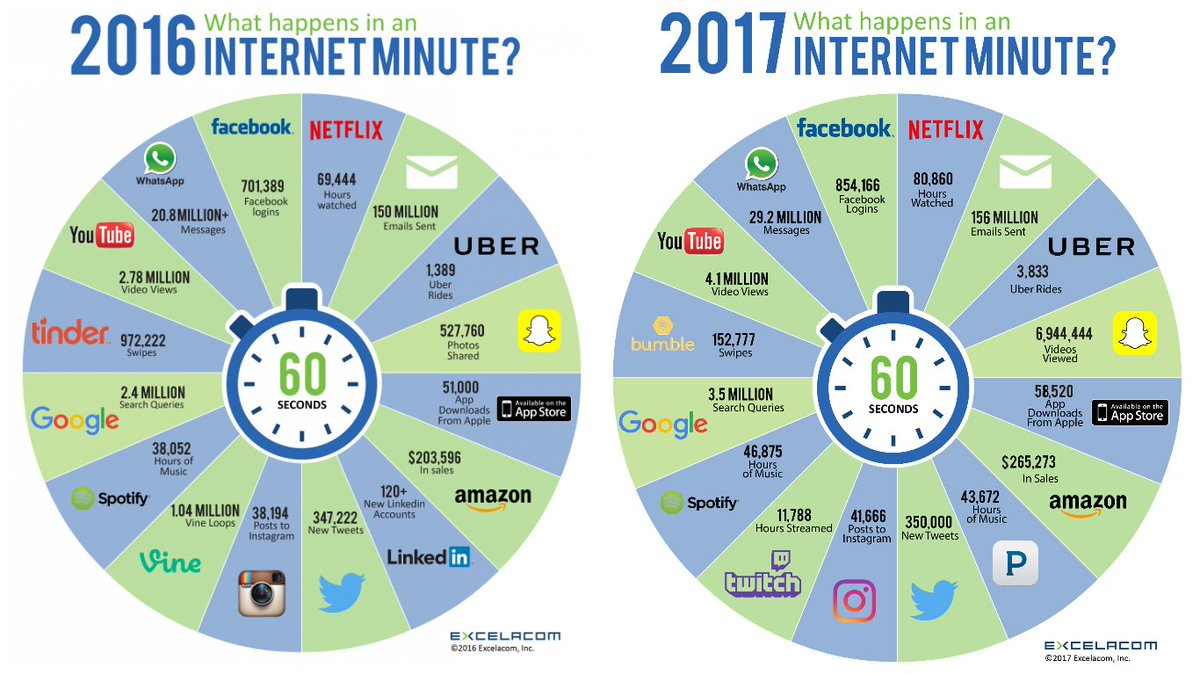
\includegraphics[width=0.80\linewidth]{figures/acontecimentoBigdata}}
		\caption{Comparação entre os anos de 2016 e 2017 do que acontece na internet a cada 60 segundos}
		\small{Fonte - (EXCELACOM, 2017)}
		\label{Fig:testeAcontecimento}
	\end{center} 
\end{figure}

Tudo isso sem contar com a IoT, onde, mais e mais dados são gerados, com sensores, leitores de RFID, smartTV, notebooks, smartphones, carros, entre outros dispositivos que geram e transmitem dados por meio da rede.

Para que a computação desta grande quantidade de informações seja realizada em tempo viável, cada vez mais faz-se necessária a exploração de paradigmas de programação paralela e processamento distribuído. Porém, desenvolver \textit{softwares} para ambientes distribuídos é uma tarefa complexa, pois envolve uma série de conceitos e problemas que devem ser considerados pelos programadores; como concorrência, tolerância a falhas, distribuição de dados e balanceamento de carga (KOLBERG, 2010).

Para armazenar e processar uma quantidade enorme de dados, foi criado o Apache Hadoop (APACHE, 2018), que é um \textit{framework} composto basicamente por dois modulos, o MapReduce para o processamento de dados de forma distribuída e o HDFS que é um sistema de arquivos escalonável e distribuído, cujo desenho é baseado fortemente no GFS (IMASTERS, 2014).

%melhorar esse parágrafo, esta muito confuso
Nas grandes empresas como Facebook, Google e Amazon, pesquisas que envolvem grandes volumes de dados, marketing direcionado, essas pesquisas são realizadas com os dados que os próprios usuários produzem. Com isso, surge alguns questionamentos. Será que os usuários sabem que seus dados estão sendo utilizados por essas empresas? Será que esses dados estão sendo armazenados de forma segura? Quais são as garantias que as empresas fornecem aos seus usuários em caso de roubo dos dados? Quais são as boas práticas de segurança utilizadas por essas empresas?

\section{Segurança em Big Data}

Nos dias de hoje, a informação passou a ser um dos bens mais preciosos das grandes organizações mundiais, não é por acaso, que os Estados Unidos espionava todos os outros paises, incluindo o Brasil, esse episódio veio a público com a revelação de um ex-técnico da CIA, conhecido como Edward Snowder em 2013 (G1, 2014).

A segurança da informação é indispensável para qualquer empresa que utiliza a tecnologia em seu dia a dia. Prevenir desastres, como perda de dados importantes ou até sofrer algum tipo de invasão de \textit{hackers}, é uma grande preocupação para os gestores (SANTOS, 2017).
Para uma boa gestão de segurança da informação é recomendado seguir em três pilares fundamentais da segurança, segundo a (NBR ISO-27002, 2013) são eles: integridade, responsável por assegurar que o conteúdo da mensagem não foi alterado, a disponibilidade, responsável por garantir que as informações estão sempre acessíveis, e a confidencialidade, responsável por assegurar o acesso à informação apenas por pessoas autorizadas.



\begin{comment}
\begin{itemize}
\item \textbf{Confidencialidade:}
A confidencialidade trata da imposição de limites de acesso à informação apenas às pessoas e/ou entidades autorizados por aqueles que detêm os direitos da informação. Ou seja, somente pessoas confiáveis podem acessar, processar e modificar os dados.\\

\item \textbf{Integridade:}
A integridade diz respeito à garantia de que as informações manipuladas conservarão todas as suas características originais. Ou seja, os dados vão se manter íntegros, conforme criados ou estabelecidos pelo proprietário.\\

\item \textbf{Disponibilidade:}
Já a disponibilidade é a garantia de que as informações estarão sempre disponíveis para o uso legítimo. Ou seja, as pessoas e/ou entidades autorizadas pelo detentor dos direitos terão sempre garantido o acesso aos dados.\\
\end{itemize}
\end{comment}

Conhecendo os pilares da segurança da informação podem-se utilizar ferramentas e mecanismos para auxiliar a segurança dos dados, dividindo-os em controle físico e controle lógico. Os controles físicos são portas, salas reservadas com seguranças, ou seja, o objetivo é proteger o ambiente físico onde encontram-se os dados, enquanto que, os controles lógicos baseiam-se em boas práticas de segurança. De acordo com (LUCENA, 2017) os controles lógicos podem ser as seguintes práticas: Criptografia, assinatura digital, honeyPot e controle de acesso.
%(Felipe Lucena SEGURANÇA DE DADOS: TUDO QUE VOCÊ PRECISA SABER 6/01/2017)

\begin{comment}
\begin{itemize}
\item \textbf{Criptografia:} Mecanismo de segurança que utiliza esquemas matemáticos e algoritmos para codificar os dados em textos inelegíveis, os quais só podem ser decodificados ou descriptografados pelas pessoas que possuem a chave de acesso.\\
\item \textbf{Assinatura digital:} Conjunto de dados criptografados, associados a um documento do qual sua função é garantir a integridade do documento, mas não a sua total confidencialidade.\\
\item \textbf{HoneyPot:} Esse é o nome dado a um software usado para detectar ou impedir ações de crackers, spammers ou qualquer outro agente externo não autorizado. Essa solução 'engana' o agente externo, fazendo-o acreditar que ele está de fato explorando uma vulnerabilidade.\\
\item \textbf{Controle de acesso:} O controle de acesso consiste em limitar o acesso a devidos usuários, de acordo com seu cargo ou conhecimento e importância dentro da organização.
\end{itemize}
\end{comment}

Existem diversas outras práticas que podem ser aplicadas nestes ambientes, como por exemplo, um \textit{firewall}, um antivírus, e entre outras técnicas específicas para ambientes diversos.

\section{Motivação}

Como explicado anteriormente, a grande quantidade de dados gerados no planeta são de extrema importância para governos e empresas, pois com os dados podem-se extrair muitas informações e com isso decisões são tomadas, sendo assim, é de suma importância que esses dados sejam protegidos de forma correta, o ambiente no qual armazena e processa os dados também deve ser protegido, com uma segurança que preveja as falhas e consiga manter os dados seguros.

Há atualmente diversas soluções tecnológicas que não habilitam quesitos mínimos de segurança durante o processo de instalação e de configuração do produto (BORDINI, 2016). Considerando que uma dessas aplicações é o Apache Hadoop, no qual a segurança não vem habilitado por \textit{default} e que há diversos tipos de riscos associados com o crescente uso de soluções de Big Data por parte das empresas, como a exposição de dados sensíveis e confidenciais na internet e o comprometimento dessas bases de dados com a exclusão, inclusão ou modificação de informações. Um estudo das vulnerabilidades de segurança no ambiente Apache Hadoop, então, pode determinar falhas de segurança e com isso boas práticas podem ser tomadas para se evitar transtornos para as empresas e usuários.

Uma maneira de estudar a segurança em Big Data utilizando o ambiente Apache Hadoop é, implementar um cenário de testes, verificar as possíveis falhas de comunicação e seu comportamento mediante ataques. Sendo assim, houve uma necessidade de montar um ambiente para que os testes pudessem ocorrer, justificando a necessidade de configurar diferentes cenários e utilizar ferramentas de invasão.

\section{Objetivos}

O Big Data, hoje em dia, mudou a forma de pensar das grandes empresas, pois as empresas detêm de muitas informações para comercializar seus produtos, como dados estatísticos, quem comprar mais, faixa etária, redes sociais, quantos cliques naquele determinado anúncio, então, isso tudo está sendo processado e está gerando infomações para que se possa lançar novas estratégias de marketing. Não só o comércio está sendo beneficiado com o grande volume de dados, o mercado financeiro, a área da saúde, e entre outras áreas.

O objetivo deste trabalho é investigar a segurança utilizada no ambiente Apache Hadoop, no qual, os dados estão armazenados e processados de forma distribuída, considerando que os dados são de extrema importância e que são valiosos, sendo assim, o trabalho propõe boas práticas de segurança para que se possa evitar perdas ou roubos de dados, tendo em vista que empresas de tecnologias importantes, tais como: MasterCard, Facebook, Google, e entre outras utilizam o ambiente Hadoop para armazenamento e processamento de grandes volumes de dados.

Além disso, este trabalho propõe analisar de forma experimental, como o ambiente Apache Hadoop se comporta durante tentativas de ataques, como por exemplo, ao executar uma tarefa pelo Apache Hadoop e tentar atacar o ambiente, como será o comportamento do \textit{framework} durante o ataque. Sabendo que a comunicação dos nós do cluster é realizada por ssh, como conseguir o usuário e a senha ou até mesmo as chaves públicas e privadas. Quais são as maneiras de burlar a segurança imposta pelo Apache Hadoop e como protegê-lo desses ataques utilizando boas práticas de segurança.

Como metodologia para atender aos objetivos deste trabalho, foram utilizadas diversas ferramentas para a criação do ambiente Apache Hadoop, tais como: o Virtual-Box, Ubuntu-Server, Kali Linux e alguns dos seus aplicativos de invasão.


\section{Metodologia}

A metodologia aplicada para a realização da análise de vulnerabilidades em ambientes Apache Hadoop é baseada na exploração de um ambiente virtualizado. A ideia principal consiste em montar um cluster e verificar suas vulnerabilidades através do sistema operacional kali linux utilizando suas ferramentas para realizar um \textit{PenTest}.

Considerado as limitações encontradas, optou-se por escolher um ambiente virtual para simular um ambiente real, tendo em vista que as maiorias dos testes são realizados antes em ambientes virtuais para que só depois possa ocorrer em um ambiente real.

Para montar o ambiente virtualizado foram utilizados \textit{softwares} gratuitos, tais como, virtual-box, ubuntu-server, kali linux e o \textit{framework} Apache Hadoop. Após montar o ambiente de teste, foram executadas algumas tarefas com o \textit{framework}, para ter a certeza de que a aplicação estava funcionando corretamente. Logo após constatar que tudo estava corretamente configurado, foi a vez de instalar e configurar o Kali linux.

Considerando que a metodologia aplicada neste trabalho é a exploração a um ambiente virtualizado, foram realizados alguns testes de invasão ao cluster, seguindo a ordem de um \textit{PenTest}, na qual obedece as etapas de reconhecimento, varredura, obtenção de acesso e obtenção das informações.

A figura \ref{Fig:EstruturaGeraldoAmbiente} apresenta a estrutura do ambiente, para uma melhor compreensão deste trabalho. Como explicado anteriormente, tanto o cluster quanto o kali linux estão na mesma rede facilitando assim a realização do \textit{PenTest}, com isso foi possível realizar ataques ao cluster.

A partir das informações da rede foi possível pensar em alguns tipos de ataque ao cluster e com isso analisar o comportamento do mesmo ao ser atacado por um usuário externo, com a utilização do \textit{software} nmap, foi possível scanear toda a rede e com isso analisar as portas abertas e as vulnerabilidades encontradas.

\begin{figure}[htbp!] 
\begin{center}
% fbox faz uma borda ao redor do seu argumento
\fbox{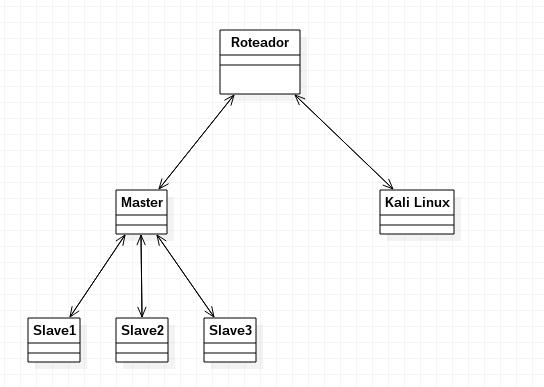
\includegraphics[width=0.80\linewidth]{figures/ClusterMelhor}}
\caption{Infográfico - Visão geral do ambiente }
\small{Fonte - (próprio autor, 2018)}
\label{Fig:EstruturaGeraldoAmbiente}
\end{center} 
\end{figure}

Pensando nas possibilidades encontradas foram sugeridos alguns ataques que poderiam levar a algum resultado significativo, os mesmos são explicados nas próximas seções.  


\subsection{Ataque de negação de serviço}
Considerando que o Apache Hadoop é um \textit{framework} resiliente a falhas, ou seja, ele saberá se comportar diante de uma falha, como por exemplo, caso um nó não funcione corretamente, os outros são capazes de suprir a necessidade, redistribuindo as tarefas para os demais nós. Então, sabendo disso, um dos ataques mais efetivos para testar isso é o ataque DoS, ou seja, apenas uma máquina atacando um nó do cluster, tentando 'derrubá-lo'.

\subsection{Ataque de força bruta}
Uma outra preocupação na utilização do \textit{framework} Apache Hadoop é que a comunicação entre os nós é realizada pelo protocolo ssh, após realizar um \textit{scanner} na rede foi possível observar que a porta 22 dos nós estavam aberta e com isso surgiu a ideia de conseguir acessar um nó através de um outro terminal remotamente.

\subsection{Ataque \textit{Man in the middle}}
Por fim, surge a ideia de realizar um \textit{man in the middle}, ou seja, ficar no meio da comunicação entre os nós, esse ataque consiste em poluir a tabela ARP da vítima induzindo ela a responder e fazer suas requisições para a máquina atacante e com isso enganá-lo.

\section{Estrutura do trabalho}

Além deste capítulo introdutório, este trabalho está organizado em mais 4 capítulos. No capítulo 2 aborda a fundamentação teórica necessária para a compreensão do trabalho. O capitulo 3 está sendo apresentado o cenário utilizado, no capitulo 4 será abordado os experimentos e resultados e o capitulo 5 a conclusão. %VOLTAR AQUI QUANDO TERMINAR O TRABALHO PARA DETERMINAR A ESTRUTURA DO TRABALHO.

\chapter{Fundamentação teórica}
\label{CAP2}

Neste capítulo serão abordados os conhecimentos necessários para a compreensão e entendimento sobre Big Data, Hadoop e a importância deles para os dias atuais, serão apresentados conceitos de Big Data, banco de dados, Hadoop e segurança dos dados em Big Data.

\section{Big Data}
\label{BigData}

Big Data é o termo usado para definir grandes volumes de dados. Esses dados são armazenados e processados para que se possam gerar resultados e poder tomar decisões. Governos , Empresas e especialistas utilizam dos dados para prever algumas situações, como por exemplo o Facebook, ele utiliza os dados dos seus usuários para traçar um perfil dele e com isso poder direcionar propagandas de marketing, a Google também consegue fazer isso de acordo com suas pesquisas e seus cliques em sites diversos, a Amazon também possui um sistema de recomendações.

Embora tenha nascido na década de 1990, o termo Big Data começou a ser desenvolvido e utilizado pelo mercado com mais frequência nos últimos anos. Muita gente, entretanto, ainda tem dúvidas sobre o seu real significado, além de sua eficácia e aplicabilidade nos negócios (EXAME, 2013).

\begin{figure}[htbp!] 
	\begin{center}
		% fbox faz uma borda ao redor do seu argumento
		\fbox{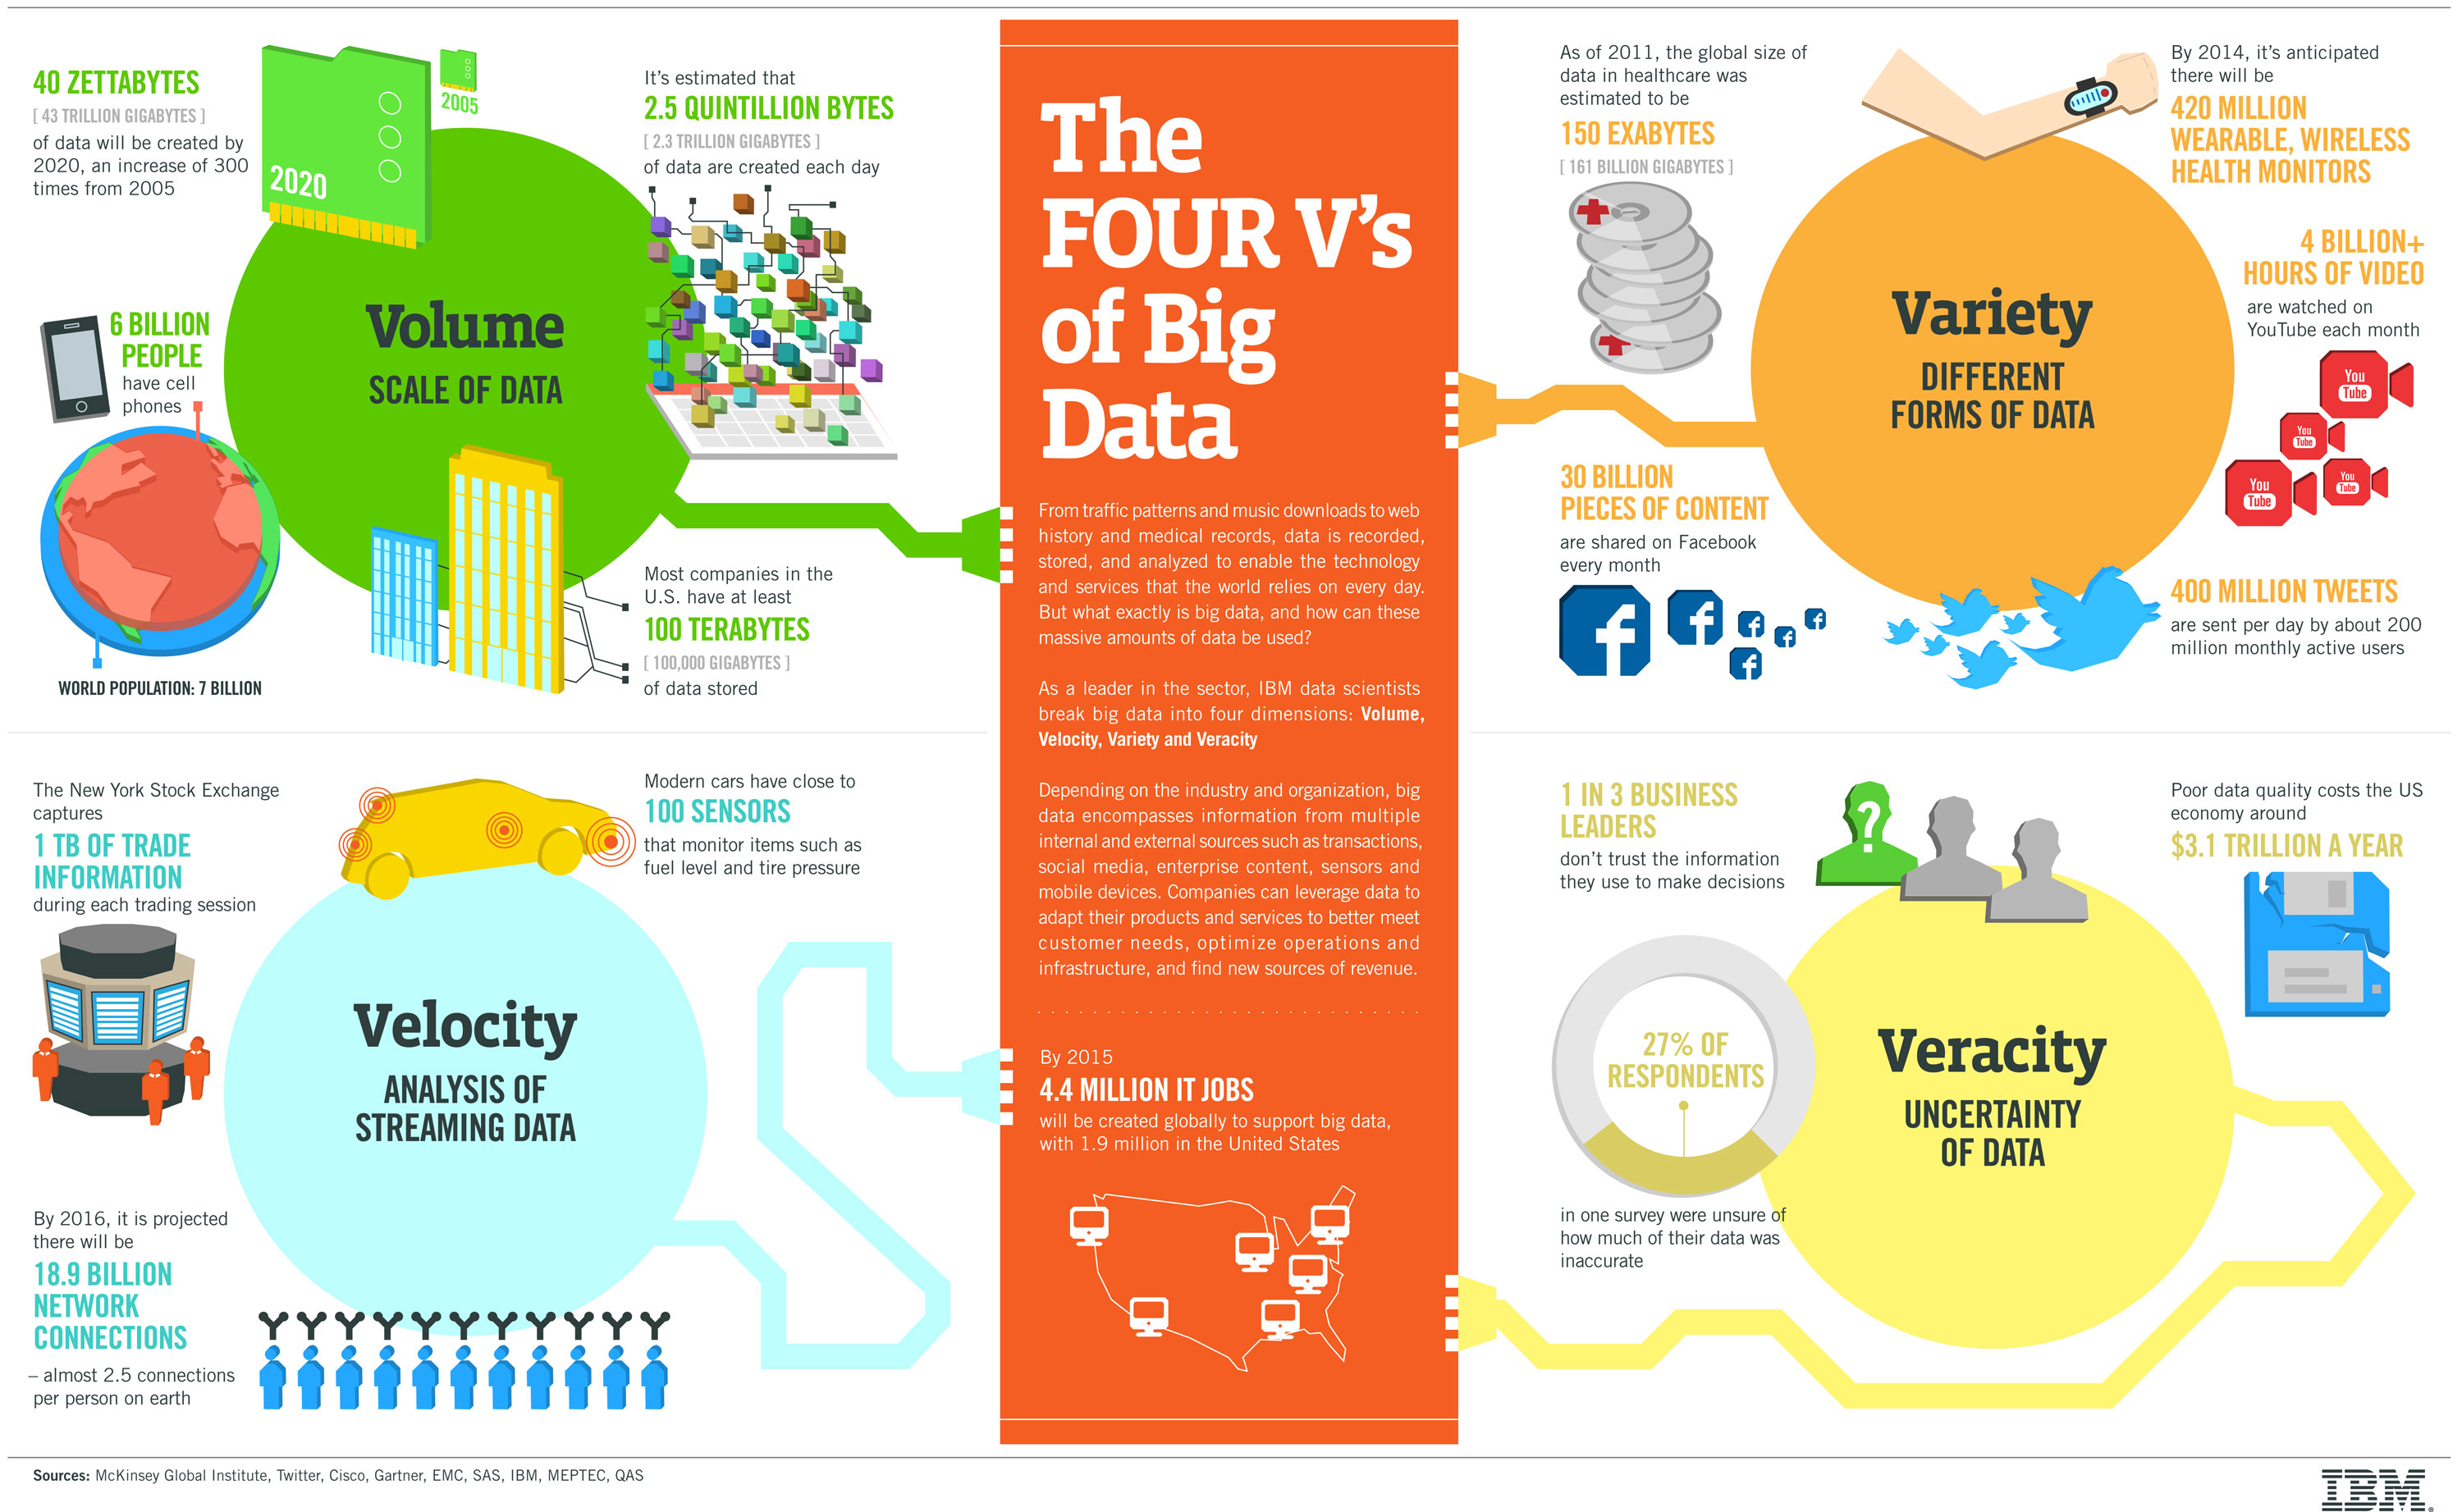
\includegraphics[width=0.80\linewidth]{figures/4-Vs-of-big-data}}
		\caption{Infográfico - The Four V's of Big Data}
		\small{Fonte - (IBM, 2014)}
		\label{Fig:4-Vs-IBM}
	\end{center} 
\end{figure}


A figura \ref{Fig:4-Vs-IBM} mostra que a IBM define Big Data como os 4v's, correspondentes a Volume, Variedade, Velocidade e Veracidade, enquanto que, alguns autores definem o termo Big Data com 5v's, adicionando o termo Valor, porém, isso ainda não é uma unanimidade, tendo em vista que o termo valor é aquilo que se extrai do Big Data, ou o que se espera extrair. Sendo assim, os 4V's são definidos da seguinte forma:

\begin{itemize}

\item \textbf{Volume:} Organizações coletam dados de uma grande variedade de fontes, incluindo transações comerciais, redes sociais e informações de sensores ou dados transmitidos de máquina a máquina.\\

\item \textbf{Velocidade:} Os dados fluem em uma velocidade sem precedentes e devem ser tratados em tempo hábil. Tags de RFID, sensores, celulares e contadores inteligentes estão impulsionando a necessidade de lidar com imensas quantidades de dados em tempo real, ou quase real.\\

\item \textbf{Variedade:} Os dados são gerados em todos os tipos de formatos de dados estruturados, dados numéricos em bancos de dados tradicionais, até documentos de texto não estruturados, e-mail, vídeo, áudio, dados de cotações da bolsa e transações financeiras.\\

\item \textbf{Veracidade:} É a lógica dos dados, necessidade de saber se os dados fazem sentido e saber da sua autenticidade.\\
\end{itemize}
%(SCHONBERGER;CUKIER, 2013, pag. 4)
Para Schonberger e Cukier (2013, pag. 4) "o Big Data se refere a trabalhos em grande escala que não podem ser feitos em escala menor, para extrair novas ideias e criar novas formas de valor de maneiras que alterem os mercados, as organizações, a relação entre cidadão e governos, e entre outros". Tendo em mente o conceito de Big Data, pode-se entender a relação que tem com os bancos de dados da seguinte forma.

\subsection{Banco de dados}

Bancos de dados são os locais que recebem e armazenam os dados. Eles estão em todas as plataformas e serviços, pois os mesmos precisam armazenar informações (TOTALCROSS, 2012). Existem muitos tipos de banco de dados, nos quais podem ser classificados em RDBMS e NoSQL, essa classificação depende de como os dados estão sendo armazenados.

Os bancos de dados relacionais estão organizados em tabelas, onde essas tabelas estão organizadas em forma de linhas e colunas, quando os dados estão sendo armazenados, há uma necessidade de criar o \textit{schema} antes do armazenamento. As relações entre as tabelas ocorrem por meio das chaves primárias e as chaves estrangeiras. Isso difere dos bancos de dados não relacionais, pois o mesmo não existe uma estrutura certa de armazenamento, não há necessidade de criar um \textit{schema} antes, os bancos de dados não relacionais possuem alta performance e escalabilidade, pois todas as informações estão armazenadas em um único registro, onde para acessar as informações são realizadas buscas por chave e valor. Considerando que os bancos de dados não relacionais não possuem uma estrutura definida para armazenar seus dados, eles são ideias para a utilização de Big Data, tendo em vista que o conteúdo de Big Data não tem formato definido.

\subsection{Cluster}

Com a enorme quantidade de dados existentes para serem processados, seria inviável processá-los em uma única máquina, ou seja, existe a necessidade de utilizar o máximo de processadores possíveis para executar essa tarefa em tempo hábil e sem grandes custos. 
	
Com isso surge o chamado cluster, que consiste em uma estrutura computacional formada por várias máquinas, na qual sua função é processar os dados de forma distribuída. 

Existem vários tipos de cluster, cada um com uma funcionalidade ou voltado para uma determinada tarefa, são eles: cluster de alto desempenho, cluster para balanceamento de carga, cluster de alta disponibilidade (INFOWESTER, 2013). Pode ocorrer a combinação de clusters no caso do Hadoop o cluster é utilizado para armazenamento e processamento de dados de forma distribuída.


\section{Apache Hadoop}
\label{Apache Hadoop}

Hoje em dia, graças à internet, a evolução dos sistemas computacionais e a informatização, as grandes empresas criam e armazenam grandes quantidades de dados, porém esses dados precisam ser processados em tempo hábil, para que se possa tomar decisões, pois aquilo que não pode ser medido não pode ser gerenciado (KAPLAN; NORTON, 1997). Se uma empresa conseguir medir seus resultados, conseguir gerenciar seus dados, com certeza sairá na frente das demais e com isso poderá alavancar seus negócios.

O Hadoop é um projeto open-source da Apache Software Foundation que visa proporcionar  computação distribuída, escalável e confiável. Conforme a Apache, o Hadoop é um \textit{framework} que permite o processamento distribuído de grandes conjuntos de dados, por meio de clusters de computadores usando modelos de programação simples, podendo funcionar em um único servidor ou em até milhares de máquinas, cada uma disponibilizando armazenamento e processamento computacional local. Além disso, o Hadoop foi concebido para detectar e tratar falhas na camada de aplicação, fornecendo um serviço altamente disponível sob um conjunto de computadores, todos propensos a falhas (APACHE, 2018).

Considerando o baixo custo, quantidade de dados gerados, a flexibilidade e escalabilidade algumas empresas começaram a utilizar o Hadoop, tais como: Amazon, Facebook, Google, IBM, Intel, Oracle, Yahoo, e entre outras. Tendo em vista que o Hadoop foi projetado para servidores de \textit{hardware} comum, reduzindo os custos dos clusters. O Hadoop é escrito na linguagem de programação java o que permite uma fácil instalação e portabilidade nas máquinas.

Considerando que o Hadoop é um projeto mantido pela Apache Software Foundation, ela também mantém diversos outros projetos que trabalham com armazenamento e processamento distribuído e que podem ser também incluídos no ambiente Hadoop, segundo a definição da própria Apache em sua página \url{hadoop.apache.org}, os outros projetos são definidos da seguinte forma:

\begin{itemize}
\item \textbf{Ambari:} Uma ferramenta baseada na web para provisionamento, gerenciamento e monitoramento de clusters do Apache Hadoop que inclui suporte para Hadoop HDFS, Hadoop MapReduce, Hive, HCatalog, HBase, ZooKeeper, Oozie, Pig e Sqoop. O Ambari também fornece um painel para visualizar a integridade do cluster, como heatmaps e capacidade de visualizar visualmente os aplicativos MapReduce, Pig e Hive, juntamente com recursos para diagnosticar suas características de desempenho de uma maneira amigável ao usuário.

\item \textbf{Avro:} Um sistema de serialização de dados.

\item \textbf{Cassandra:} Um gerenciador de bando de dados escalável, que possui múltiplos nós mestres e portanto não apresenta um ponto de falha único.

\item \textbf{Chukwa:} Um sistema de coleta de dados para gerenciar grandes sistemas distribuídos.

\item \textbf{Hbase:} Um sistema de gerenciador de banco de dados escalável e distribuído, para o armazenamento de Big Data.

\item \textbf{Hive:} Um \textit{software} de data \textit{warehouse} para consultas e gerenciamento de grandes conjuntos de dados armazenados em sistemas de arquivos distribuídos.

\item \textbf{Mahout:} Uma biblioteca escalável para o aprendizado de máquinas e \textit{data mining}.

\item \textbf{Pig:} Uma plataforma para análise de grandes bases de dados, que consiste de uma linguagem de alto nível para expressar programas visando a análise de dados.

\item \textbf{Spark:} Um mecanismos rápido e geral para o processamento de dados em larga escala.

\item \textbf{Tez:} Uma estrutura de programação de fluxo de dados generalizada, criada no Hadoop Yarn, que fornece um mecanismo poderoso e flexível para executar um DAG arbitrário de tarefas para processar dados para casos de uso em lote e interativos. O Tez está sendo adotado pelo Hive, Pig e outras estruturas no ecossistema Hadoop e também por outros \textit{softwares} comerciais para substituir o Hadoop MapReduce como o mecanismo de execução subjacente.

%\nomenclature[ag]{YARN}{Yet Another Resource Negotiator}
%\nomenclature[al]{DAG}{directed acyclic graph}
%\nomenclature[am]{ETL}{Extract Transform Load (Extração Transformação Carregamento)}


\item \textbf{ZooKeeper:} Um serviço centralizado para manter informações de congurações, que proporciona sincronização distribuída e serviços de grupo.
\end{itemize}

O Apache Hadoop é um \textit{framework} para processamento e armazenamento distribuído, isso é realizado graças a os dois principais subprojetos do Apache Hadoop, o Hadoop HDFS e o Hadoop MapReduce, dos quais são explicados a seguir.

\subsection{Hadoop HDFS}

O HDFS — um subprojeto do projeto Apache Hadoop — é um sistema de arquivos altamente tolerante a falhas projetado para executar em \textit{hardware} padrão de baixo custo (HANSON, 2013).
Como sabe, o Apache Hadoop é indicado para armazenamento de grande quantidades de dados, na casa dos pentabytes, e com isso o sistema de arquivos utilizado é o HDFS. O HDFS permite a conexão com os nós, esses nós são os computadores de baixo custo, formando um cluster, onde os dados são distribuídos. 

Segundo o Tom White (2015, pag. 45), o HDFS é um sistema de arquivos distribuído destinado ao armazenamento de grandes arquivos chegando a terabytes com fluxos de acesso a dados padronizados, executado em clusters de servidores comuns. De certo modo, as definições do HDFS, seguem o mesmo padrão, ou seja, é um sistema de arquivo que suporta grandes quantidades de dados e é tolerante a falhas. O HDFS têm muitas similaridades com outros sistemas de arquivos distribuídos, mas é diferente em vários aspectos. Uma diferença notável é o modelo WORM do HDFS que 'afrouxa' as exigências do controle de simultaneidade, simplifica a persistência de dados e habilita acesso de alto rendimento (HANSON, 2013), ou seja, o HDFS é ideal para aplicações que realizam poucas escritas e muitas leituras.%(HANSON, 2013,IBM)
%\nomenclature[af]{WORM:}{write-once-read-many}%

No HDFS, os arquivos são divididos em blocos e replicados em vários nós, e mesmo sendo executado em \textit{hardware} comum e sujeito a falhas de máquinas, o HDFS disponibiliza replicação, detecção de falhas e recuperação de blocos de dados, automaticamente, mantendo a integridade do sistema de arquivos (BRITO, 2014).

\subsubsection{Arquitetura do Hadoop HDFS}

O HDFS segue uma estrutura de mestre e escravo onde o mestre atribui tarefas aos escravos. Os componentes do Hadoop HDFS são:

\begin{itemize}
	\item \textbf{NameNode:}
    Tem como responsabilidade gerenciar os arquivos armazenados no HDFS. Suas funções incluem mapear a localização, realizar a divisão dos arquivos em blocos, encaminhar os blocos aos nós escravos, obter os metadados dos arquivos e controlar a localização de suas réplicas. Como o NameNode é constantemente acessado, por questões de desempenho, ele mantém todas as suas informações em memória. Ele integra o sistema HDFS e fica localizado no nó mestre da aplicação.
	
    \item \textbf{DataNode:}
    Enquanto o NameNode gerencia os blocos de arquivos, são os DataNodes que efetivamente realizam o armazenamento dos dados. Como o HDFS é um sistema de arquivos distribuído, é comum a existência de diversas instâncias do DataNode em uma aplicação Hadoop, para que eles possam distribuir os blocos de arquivos em diversas máquinas. Um DataNode poderá armazenar múltiplos blocos, inclusive de diferentes arquivos. Além de armazenar, eles precisam se reportar constantemente ao NameNode, informando quais blocos estão guardando bem como todas as alterações realizadas localmente nesses blocos.

	\item \textbf{Bloco de arquivos}
    Em geral, os dados do usuário são armazenados nos arquivos da HDFS. O arquivo em um sistema de arquivo será dividido em um ou mais segmentos ou dados armazenados em cada um nós. Esses arquivos são chamados segmentos como blocos. Em outras palavras, o montante mínimo de dados que HDFS pode ler ou escrever é chamado de bloco. O tamanho de bloco padrão é de 64MB, mas pode ser aumentada conforme a necessidade de mudança na configuração HDFS.
    
    \item \textbf{Namespace}
    O HDFS suporta uma organização hierárquica tradicional de arquivos em que um usuário ou um aplicativo pode criar diretórios e armazenar arquivos neles. A hierarquia do namespace do sistema de arquivos é similar à maioria dos outros sistemas de arquivos existentes; é possível criar, renomear, reposicionar e remover arquivos.
    

	\item \textbf{SecondaryNameNode:}
    Utilizado para auxiliar o NameNode a manter seu serviço, e ser uma alternativa de recuperação no caso de uma falha do NameNode. Sua única função é realizar pontos de checagem do NameNode em intervalos pré definidos, de modo a garantir a sua recuperação e atenuar o seu tempo de reinicialização.
\end{itemize}

A figura \ref{Fig:Estrutura HDFS} mostra de maneira geral a estrutura da arquitetura do HDFS e do seu formato de trabalho. 

%link da referencia: https://lakshmana-msbi.blogspot.com.br/2016/01/big-data-hadoop-lesson-5-namenode.html

\begin{figure}[htbp!] \begin{center}
% fbox faz uma borda ao redor do seu argumento
\fbox{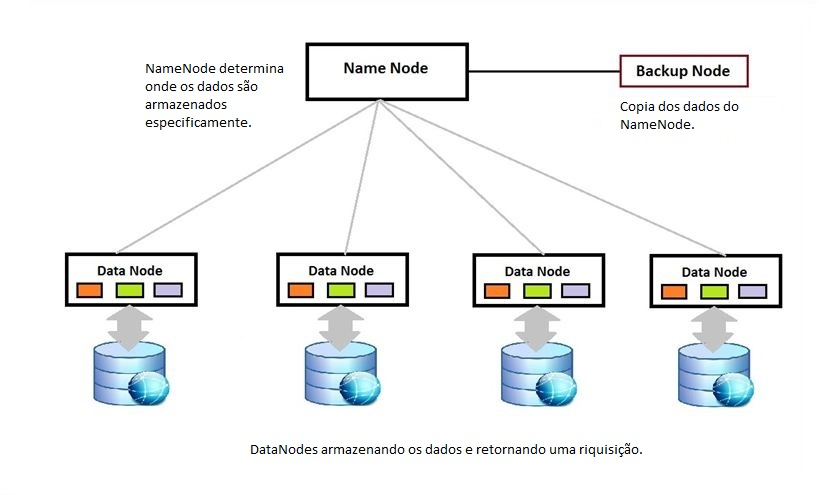
\includegraphics[width=0.80\linewidth]{figures/namenode}}
\caption{Infográfico - Visão geral HDFS }
\small{Fonte - (MSBI, 2016)}
\label{Fig:Estrutura HDFS}
\end{center} \end{figure}


\subsection{Hadoop MapReduce}

MapReduce é um modelo de programação projetado para processamento paralelo e distribuído de grandes conjuntos de dados, criado pela Google, esse paradigma distribui os dados no formato chave-valor, onde a chave é o identificador do registro e valor é o seu conteúdo.

%(LOPES,http://joseguilhermelopes.com.br/hadoop-entenda-arquitetura-hdfs/).

Um trabalho MapReduce normalmente divide o conjunto de dados de entrada em blocos independentes que são processados pelas tarefas do Map de maneira completamente paralela. A estrutura classifica as saídas dos Maps, que são inseridas nas tarefas de \textit{reduce}. Normalmente, tanto a entrada quanto a saída do \textit{Job} são armazenadas em um sistema de arquivos. O \textit{framework} cuida das tarefas de planejamento, monitora-as e re-executa as tarefas com falha (APACHE,2018).

Para Tom White (2015, pag.19 e 22), o MapReduce é um modelo de programação para processamento de dados e que o MapReduce funciona dividindo o processo em duas partes, ou seja, na fase Map e na fase \textit{Reduce}.

O MapReduce consegue abstrair a programação paralela em apenas duas funções, a Map e a \textit{Reduce} facilitando a vida do desenvolvedor, como demonstra a figura \ref{Fig:Estrutura Mapreduce01}.

\begin{figure}[htbp!] \begin{center}
% fbox faz uma borda ao redor do seu argumento
\fbox{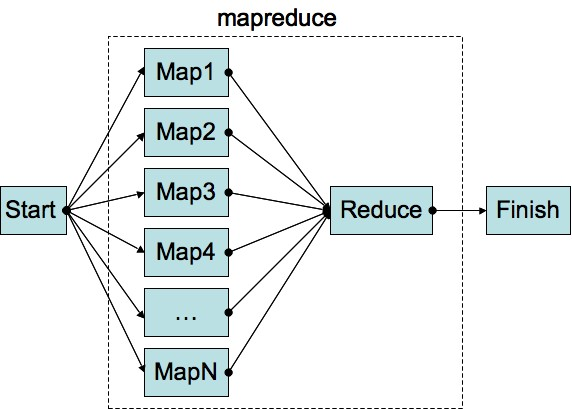
\includegraphics[width=0.60\linewidth]{figures/mapreduce}}
\caption{Infográfico - Visão geral do funcionamento do MapReduce }
\small{Fonte - (LOPES, 2016)}
\label{Fig:Estrutura Mapreduce01}
\end{center} \end{figure}


\subsubsection{arquitetura do MapReduce}

Como pode-se observar na figura \ref{Fig:Estrutura MapReduce02}, a arquitetura MapReduce é semelhante a arquitetura do HDFS, sendo também baseada em mestre e escravo, onde o JobTracker é o mestre e o TaskTracker é o escravo. Segundo Tom White (2015, pag. 83) esses dois componentes do MapReduce são definidos da seguinte forma:


\begin{figure}[htbp!] \begin{center}
% fbox faz uma borda ao redor do seu argumento
\fbox{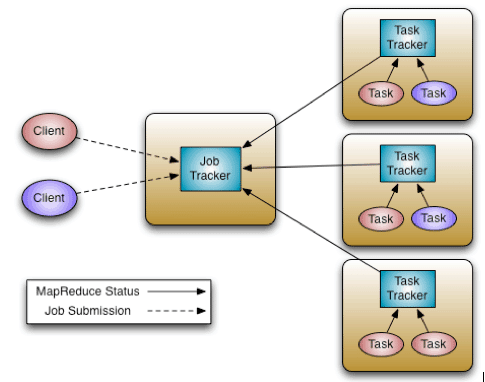
\includegraphics[width=0.80 \linewidth]{figures/mapReduce}}
\caption{Infográfico - Visão geral MapReduce }
\small{Fonte - (HORTONWORKS, 2012)}
\label{Fig:Estrutura MapReduce02}
\end{center} \end{figure}
%link da figura: 
%https://br.hortonworks.com/blog/apache-hadoop-yarn-background-and-an-overview/


\begin{itemize}
	\item \textbf{JobTracker:} Assim como o NameNode, o JobTracker também possui uma função de gerenciamento, porém, nesse caso, o controle é realizado sobre o plano de execução das tarefas a serem processadas pelo MapReduce. Sua função é designar diferentes nós para processar as tarefas de uma aplicação e monitorá-las enquanto estiverem em execução. Um dos objetivos do monitoramento é, em caso de falha, identificar e reiniciar uma tarefa no mesmo nó ou, em caso de necessidade, em um nó diferente.\\
    
    \item \textbf{TaskTracker:} Processo responsável pela execução de tarefas MapReduce. Assim como os DataNodes, uma aplicação Hadoop é composta por diversas instâncias de TaskTrackers, cada uma em um nó escravo. Um TaskTracker executa uma tarefa Map ou uma tarefa \textit{Reduce} designada a ele. Como os TaskTrackers rodam sobre máquinas virtuais, é possível criar várias máquinas virtuais em uma mesma máquina física, de forma a explorar melhor os recursos computacionais.
\end{itemize}

Apesar da solução Hadoop com HDFS e o MapReduce ser muito útil para diversas aplicações, foram encontradas algumas limitações em sua versão 1.0, segundo Tom White (2015, pag.84), o MapReduce tinha uma limitação quando se trabalhava com cerca de 4000 mil nós e 40000 mil tarefas, pois o JobTracker ficava sobrecarregado e com isso era gerado uma perda de performance em cascata, outro problema encontrado era quando o JobTracker falhasse, todo restante da aplicação, ou seja, os taskTracker também falhavam, e tudo era perdido, com isso houve a necessidade de uma atualização, dai surgiu o Yarn, o Hadoop foi atualizado para a versão 2.0 e junto com ele vem o \textit{framework} Yarn onde será explicado na próxima seção.

\subsection{Apache Hadoop YARN}

Como explicado anteriormente, o MapReduce na versão 1.0 sobrecarregava muito o JobTracker, com isso ocasionava uma falha em cascata, pois o JobTracker tinha o papel de gerenciar, monitorar e verificar falhas, sendo assim surge o \textit{Framework} Yarn, também é um \textit{framework} para trabalhar com processamento e armazenamento distribuído. O Yarn é um gerenciador de aplicativos distribuídos e de uso geral que veio pra substituir a antiga estrutura do MapReduce na qual se concentravam as taferas e o gerenciamento apenas no JobTracker. Com o Yarn, o gerenciamento que antes era realizado pelo JobTracker agora passa a ser gerenciado pelo Yarn, onde o mesmo possui uma estrutura diferenciada para tal atividade. O Yarn possui os componentes ResourceManager, NodeManager e o ApplicationMaster, todos irão executar as tarefas que antes eram executadas apenas pelo JobTracker. Segundo a Hontonworks, os componentes do Yarn são definidos da seguinte forma:




\begin{comment}
\begin{figure}[htbp!] \begin{center}
% fbox faz uma borda ao redor do seu argumento
\fbox{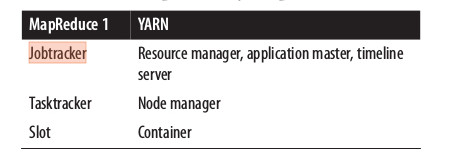
\includegraphics[width=0.80\linewidth]{figures/comparacaoYarn_mapReduce01}}
\caption{Comparação - Yarn e MapReduce 1}
\small{Fonte - (WHITE, 2015)}
\label{Fig:Comparação - Yarn e MapReduce 1}
\end{center} \end{figure}
\end{comment}



\begin{itemize}

\item \textbf{ResourceManager:}
Possui um escalonador conectável, que é responsável por alocar recursos para vários aplicativos em execução, sujeitos a restrições familiares de capacidades, filas, e entre outras. O Agendador é um agendador puro no sentido de que não realiza monitoramento ou rastreamento de status para o aplicativo, não oferecendo garantias sobre a reinicialização de tarefas com falha devido a falhas de aplicativos ou falhas de \textit{hardware}. O Agendador executa sua função de agendamento com base nos requisitos de recursos dos aplicativos; Ele faz isso com base na noção abstrata de um recipiente de recursos que incorpora elementos de recursos como memória, CPU, disco, rede, e entre outros.

\item \textbf{NodeManager:}
É o escravo por máquina, que é responsável por lançar os recipientes dos aplicativos, monitorar o uso de recursos e relatar o mesmo ao ResourceManager.

\item \textbf{ApplicationMaster:}
Tem a responsabilidade de negociar contêineres de recursos apropriados do \textit{Scheduler}, rastreando seu status e monitorando o progresso. Da perspectiva do sistema, o próprio ApplicationMaster é executado como um contêiner normal.

\end{itemize}

Como ilustra a figura \ref{Fig:Estrutura YARN}, após instalado o Yarn, tem-se uma arquitetura similar ao MapReduce versão 1.0, porém com algumas vantagens, sendo uma delas de que se o nó mestre parar de funcionar toda a aplicação ainda continua funcionando, coisa que não acontecia na versão 1.0 do Hadoop.


\begin{figure}[htbp!] \begin{center}
% fbox faz uma borda ao redor do seu argumento
\fbox{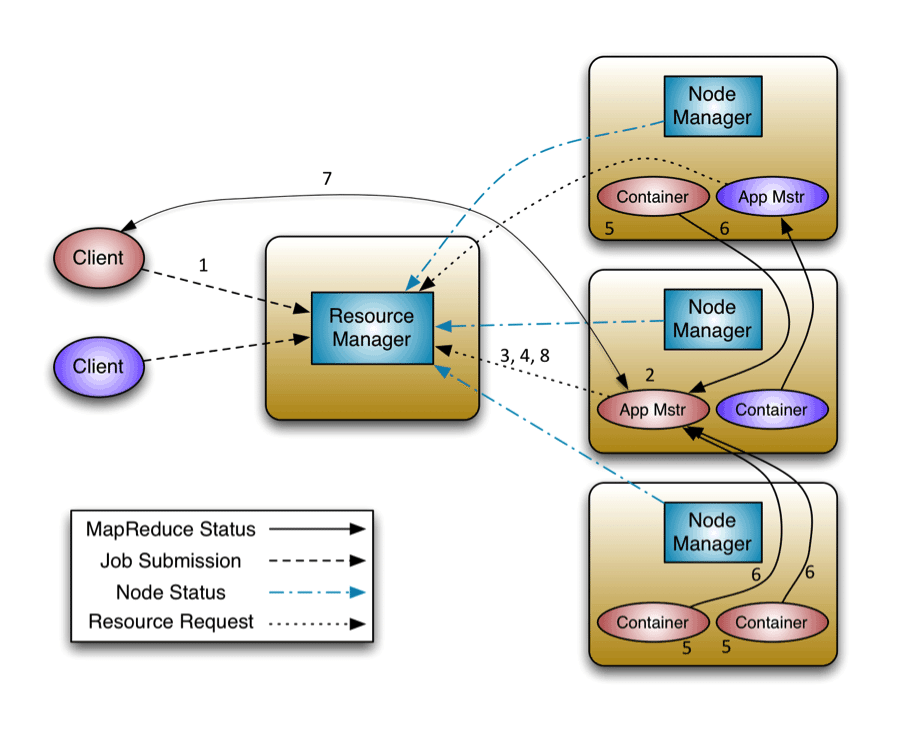
\includegraphics[width=0.80\linewidth]{figures/yarnflow}}
\caption{Infográfico - Visão geral YARN }
\small{Fonte - (Apache, 2018)}
\label{Fig:Estrutura YARN}
\end{center} \end{figure}

\newpage
\subsection{Segurança do Hadoop}

Nas versões anteriores do Hadoop a segurança fornecida é a que o cluster será utilizado por um grupo de usuários fechado, e as medidas de segurança são para evitar perdas acidentais e não autenticação (WHITE, 2015).

Com a replicação dos dados em nós diferentes, isso faz com que em casos de perda de dados, ou por descuido de algum usuário, os dados possam ser recuperados, pois existem cópias deles em outros nós. Isso não impede que usuário possa entrar como root e excluir todos os arquivos da raiz.

O que faltava para o Hadoop era um mecanismo de autenticação que garantisse que aquele usuário que estava tentando realizar tal atividade era ele mesmo (WHITE, 2015). A segurança do Hadoop é a autorização, apenas identifica se o usuário tem ou não a permissão para executar aquela tarefa desejada.

De acordo com White (2015) a autorização não é suficiente por si só, porque o sistema ainda está aberto ao abuso por meio de falsificação por um usuário mal-intencionado que pode ganhar rede e acesso ao cluster.

A instalação do Apache Hadoop não traz consigo uma segurança baseada em autenticação, com isso, faz necessário a implementação do protocolo kerberos.

\subsubsection{Protocolo Kerberos}

O Kerberos foi criado em meados dos anos 80, no instituto de tecnologia de Massachusetts, por Clifford Neuman e Steve Miller, ele foi desenvolvido durante durante o Projeto Athena, usando como base o protocolo Needham-Schroeder (LUZ, 2011).
%https://www.profissionaisti.com.br/2011/11/conhecendo-o-protocolo-de-rede-kerberos/
A ideia principal do protocolo é evitar a entrada de usuários estranhos na rede, ou seja, só entra usuários autenticados, e a autenticação do protocolo funciona por três serviços, três servidores. 
%https://www.gta.ufrj.br/grad/02_2/kerberos/

\begin{itemize}

\item \textbf{Servidor de Autenticação (SA):} Responsável pela autenticação em si do usuário, pois a partir de um pedido a este servidor, ele receberá um ticket e uma chave de sessão, podendo assim continuar tentando se conectar com o sistema.\\

\item \textbf{Servidor de Concessão de Ticket (TGS):} É o responsável pela concessão dos tickets para os serviços que utilizam o Kerberos.\\

\item \textbf{Servidor de Administração (KADM):} Responsável pelo controle das chaves secretas, cadastrando-as tanto no cliente quanto no servidor. Para isso o usuário precisa fazer o seu cadastramento, escolhendo um username e uma senha.\\

\end{itemize}

\begin{figure}[htbp!] 
\begin{center}
% fbox faz uma borda ao redor do seu argumento
\fbox{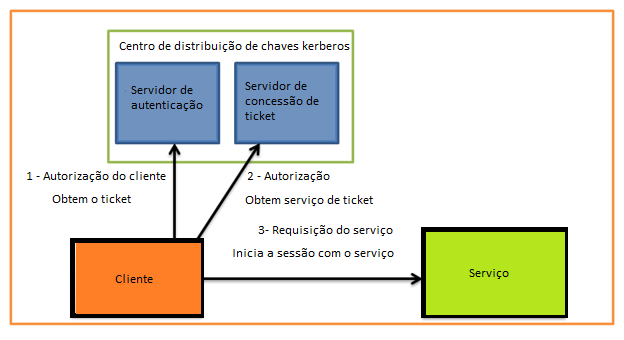
\includegraphics[width=0.80\linewidth]{figures/funcionamentoKerberos}}
\caption{Visão do funcionamento do kerberos }
\small{Fonte - (DROIDHUB, 2014)}
\label{Fig:Visão do funcionamento do kerberos}
\end{center} 
\end{figure}

O funcionamento do kerberos possui muitas vantagens, uma delas é que as senhas duram poucas horas, ao realizar uma requisição ao servidor de autenticação e depois ao servidor de concessão de ticket o usuário garente uma senha, porém ela dura por no máximo 8 horas, dificultando assim alguma tentativa de força bruta. 

Muitas aplicações podem ser protegidas pelo kerberos, tais como: ssh, telnet, linux, e entre outros. A figura \ref{Fig:Visão do funcionamento do kerberos} ilustra uma visão geral do funcionamento do protocolo kerberos, demonstrando que antes de tudo o cliente faz uma requisição para os servidores kerberos e logo após isso é que terá acesso ao servidor, que pode ser um ambiente Hadoop.

\section{Tipos de ataques à segurança}

Nos dias de hoje existem milhares de ataques diferentes, porém, neste trabalho foram utilizados três dos mais conhecidos no mundo da segurança da informação, eles são simples na sua forma de execução, mas o resultado pode ser desastroso para a vítima, sendo assim, são eles:
%\nomenclature[da]{DOS:}{Denial Of Service}%

\begin{itemize}
\item \textbf{DoS:} É uma tentativa de fazer com que aconteça uma sobrecarga em um servidor ou computador comum para que recursos do sistema fiquem indisponíveis para seus utilizadores (CANALTECH, 2018). Essa prática de ataque não tem a intenção de invadir o sistema, mas tem a pretensão de deixar o sistema indisponível para os usuários, enviando muitos pacotes de requisições, na qual irá sobrecarregar a vítima, pois ela não irá conseguir responder todas as requisições e com isso irá ficar indiponível.\\
%https://canaltech.com.br/produtos/O-que-e-DoS-e-DDoS/

Ataques DDoS são executados há tempos e já prejudicaram empresas bastante conhecidas. Historicamente, servidores da CNN, Amazon, Yahoo, Microsoft e eBay já foram "vítimas". Em dezembro de 2010, por exemplo, os sites da Visa, Mastercard e Paypal sofreram ataques DDoS de um grupo defendendo a não existência de "censura" na internet. Em fevereiro de 2012, ataques foram executados contra sites de bancos brasileiros por motivos semelhantes (ALECRIM, 2012).\\
%https://www.infowester.com/ddos.php

\begin{figure}[htbp!] 
\begin{center}
% fbox faz uma borda ao redor do seu argumento
\fbox{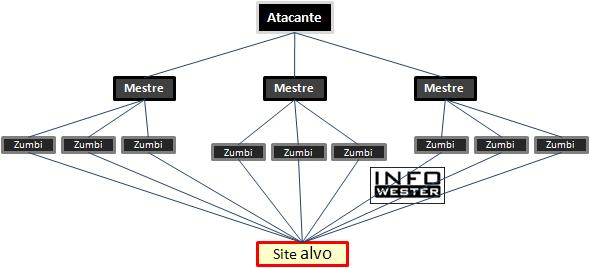
\includegraphics[width=0.80\linewidth]{figures/ddos}}
\caption{Visão do funcionamento de um DDoS}
\small{Fonte - (INFOWESTER, 2012)}
\label{Fig:Visão do funcionamento de um DDOS}
\end{center} 
\end{figure}

A figura \ref{Fig:Visão do funcionamento de um DDOS} mostra uma visão geral do funcionamento de um DDoS, o ataque de negação de serviço utilizado neste trabalho consiste em apenas uma máquina enviando pacotes para outra máquina, na tentativa de sobrecarregar o serviço e assim poder visualizar seu comportamento mediante ataques.\\

\item \textbf{Metasploit framework: } Plataforma de teste de penetração modular baseada em Ruby que permite escrever, testar e executar código de exploração. O \textit{Metasploit Framework} contém um conjunto de ferramentas que pode ser usada para testar vulnerabilidades de segurança, enumerar redes, executar ataques e evitar a detecção. Em sua essência, o \textit{Metasploit Framework} é uma coleção de ferramentas comumente usadas que fornecem um ambiente completo para testes de penetração e desenvolvimento de exploração.\\
%https://metasploit.help.rapid7.com/docs/msf-overview

Esse \textit{framework} possui um conjunto de ferramentas que podem ser acessadas pelo seu console msf. Nesta aplicação foi utilizado uma das suas ferramentas de força bruta, que pode ser utilizado nos seguintes protocolos: ssh, telnet e ftp. Essa ferramenta é formada por um conjunto de \textit{exploit}, que podem encontrar vulnerabilidades diversas nos sistemas.\\

\item \textbf{Man in the middle: } Traduzindo do inglês para o português como homem no meio, significa que o atacante irá ficar entre dois terminais, ou seja, no meio da conexão entre as duas vítimas, interceptando todo tráfego de comunicação entre essas duas máquinas. Esse ataque pode ter algumas variantes, através dele pode-se clonar o browser das vítimas, enviar e-mails falsos, e entre outros. Esse ataque é muito difícil de detectar, pois ambos os usuários pensam que estão se comunicando sem que ninguém perceba. Neste trabalho foi utilizado esse ataque e com a ferramenta ettercap, foi possível conseguir poluir a tabela ARP de um host, com isso, foi possível saber que ele estava se reportando para a máquina atacante, ao invés de se reportar para a máquina verdadeira, como ilustrado na figura \ref{Fig:Visão geral do mitm}.
%http://www.webcheats.com.br/threads/6-ataque-man-in-the-middle.2552630/
%\nomenclature[db]{MITM:}{Man in the middle}%


%ajeitar a legenda
\begin{figure}[htbp!] 
\begin{center}
% fbox faz uma borda ao redor do seu argumento
\fbox{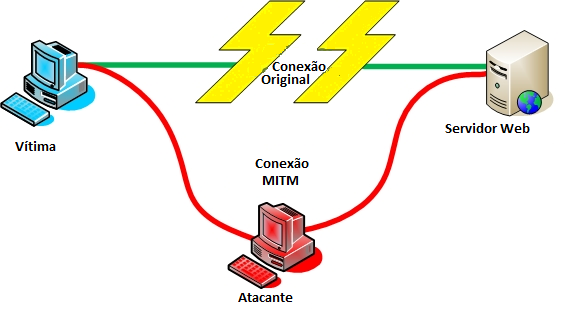
\includegraphics[width=0.80\linewidth]{figures/manInTheMiddle}}
\caption{Visão geral de um MITM }
\small{Fonte - (DARKMOREOPS, 2016)}
\label{Fig:Visão geral do mitm}
\end{center} 
\end{figure}

\item \textbf{Protocolo ARP: } O protocolo ARP é o mecanismo responsável pela associação do endereço MAC a um endereço IP, da seguinte forma: Se um hostA pretende se comunicar com um hostB, então o hostA pega o endereço IP do hostB e envia pra rede em broadcast "peguntando quem tem o endereço físico correspondente aquele IP", com isso, o hostB "responde com o endereço físico, ou seja, o endereço MAC". Dai o hostA guarda em uma tabela, a tabela ARP, o endereço IP e o endereço MAC correspondentes, e com isso pode ocorrer a comunicação (PINTO, 2011).

%\nomenclature[dc]{ARP:}{Address Resolution Protocol}%
%\nomenclature[dd]{IP:}{Internet Protocol}%
%\nomenclature[de]{MAC:}{Media Access Control}%
%https://pplware.sapo.pt/microsoft/windows/redes-sabe-para-que-serve-o-protocolo-arp/
\end{itemize}

%\newpage
\section{PenTest}

O \textit{PenTest}, também conhecido como Teste de Intrusão, é um teste realizado em uma rede ou um sistema de computadores com o objetivo de descobrir vulnerabilidades no sistema. Através desse teste um Pentester pode descobrir todas as vulnerabilidades encontradas em uma rede e até mesmo descobrir qual o tamanho do dano que uma invasão causaria aos computadores e a rede.

Existem dois tipos de \textit{PenTest}, o \textit{Blackbox} e \textit{Whitebox}, cada tipo de teste é feito para descobrir diferentes problemas e para prever diferentes tipos de ataques.

\subsubsection{Whitebox}
O \textit{Whitebox} é um teste realizado com o Pentester sabendo todas as informações sobre a rede como topografia, IPs, senhas, níveis de usuários e logins. Esse é o mais amplo de todos os testes e é capaz de encontrar qualquer vulnerabilidade.

\subsubsection{Blackbox}
O \textit{Blackbox} é um teste mais voltado para situações reais onde o testador não terá nenhuma informação sobre o sistema, quase como um teste cego.

Esse teste é muito próximo do que acontece na vida real quando um \textit{cracker} tenta quebrar a segurança de uma rede e é atualmente o mais requisitado pelas empresas. %( http://ninjadolinux.com.br/o-que-e-pentest/  ); (Cassio Augusto Fevereiro 10, 2017 )

\subsection{Fases de um PenTest}
Uma análise de \textit{PenTest} consiste em fases bem definidas e organizadas, normalmente divididas em um ciclo de vida, na qual cada fase possui diferentes etapas, definidas a seguir.

\subsubsection{Fase de Reconhecimento}
Nessa fase a equipe de PenTesters realiza o levantamento do máximo de informações possíveis sobre a empresa analisada. Dados como os serviços prestados, os principais gerentes e diretores, localização física, existência de filias, e entre outras.

\subsubsection{Fase de Varredura}
Nesse momento é realizado uma varredura do que está presente na rede. Por exemplo, o range de IPs que é utilizado, quais os servidores existentes, os sitemas operacionais utilizados, as portas abertas, e entre outras.

\subsubsection{Fase de Obtenção de Acesso e Exploração}
Com base no que foi identificado na fase de varredura, o PenTester fará a exploração de cada item, efetivamente em busca das vulnerabilidades existentes. Com o uso de técnicas de \textit{exploit} e \textit{brute force} tentará identificar quais serviços estão vulneráveis e que tipo de informação, falhas ou controles podem ser obtidos através daquele serviço.

\subsubsection{Fase de Obtenção de Evidências e Reporte}
As evidências de todas as falhas e vulnerabilidades identificadas são coletada pela equipe. Com base nessas informações, é gerado um relatório completo indicando os pontos vulneráveis de todos os elementos da empresa, falhas na rede, em \textit{software} mal configurados e desatualizados, falta de elementos de segurança, e entre outros, indicando inclusive que prejuízos podem ser causados à empresa em cada uma das falhas.
%(http://profissaohacker.com/pentest/);
%(AJEITAR ISSO AQUI)

Para realizar os teste de invasão os Pentesters utilizam diversas ferramentas e sistemas operacionais, mas o sistema mais utilizado é o kali linux, definido a seguir.

\subsection{Kali Linux}
	Uma das ferramentas mais indicadas pelos profissionais da área de segurança da informação é o Kali Linux (antigo Backtrack) que é um sistema operacional feito para \textit{hackers} e para a realização de testes de intrusão. O Kali é uma distribuição Linux, baseada em Debian que possui centenas de ferramentas para realização de testes de segurança e para exploração de vulnerabilidades (AUGUSTO, 2017).
    De acordo com a página oficial do kali linux, na sua documentação ele é definido como

\begin{flushright}
\small\it
	"O Kali Linux é uma distribuição Linux baseada no Debian destinada a testes avançados de penetração e auditoria de segurança. Kali contém várias centenas de ferramentas que são voltadas para várias tarefas de segurança da informação, tais como, testes de penetração, pesquisa de segurança, computação forense e engenharia reversa. O Kali Linux é desenvolvido, financiado e mantido pela Offensive Security, uma empresa líder em treinamento de segurança da informação" (KALI LINUX, 2018).
\end{flushright}

Além disso, ainda de acordo com a pagina oficial, o kali linux possui mais de 600 ferramentas de teste de penetração, é livre de código aberto e possui diversos suportes, tornando-se assim a ferramenta ideal e preferida para profissionais da área de segurança da informação.

%https://www.kali.org/
%(09/05/2018)

Com as ferramentas que o kali linux oferece é possivel realizar diversos tipos de testes de penetração, seguindo a ordem de um ataque que é desde o levantamento de informações até a obtenção dos dados, em cada fase dos ataques existem um conjunto de ferramentas designadas.

Dentre todas as ferramentas existentes no sistema operacional kali linux, existem algumas que merecem destaque e que são quase sempre utilizadas para realizar algum tipo de ataque, são elas:

\begin{itemize}
\item \textbf{Nmap:} A página oficial do nmap o define como
\begin{flushright}
\small \it
	"O Nmap é uma ferramenta de código aberto para exploração de rede e auditoria de segurança. Ela foi desenhada para escanear rapidamente redes amplas, embora também funcione muito bem contra hosts individuais" (NMAP, 2018).\\
\end{flushright}
%(https://nmap.org/man/ptBR/index.html) (09/05/2018)\\

\item \textbf{Wireshark:} O Wireshark é um analisador de protocolos de rede, ele analisa o tráfego da rede de forma minunciosa.\\

\item \textbf{Metasploit framework:} Esse \textit{framework} consiste de um conjunto de aplicações que são utilizadas para testes de invasão.\\

\item \textbf{Ettercap:} Mais uma ferramenta para testes de invasão, ela é muito utilizada para realizar ataque \textit{man in the middle}, ou seja, homem no meio traduzindo para o português.

\item \textbf{Aircrack-ng:} Essa ferramenta é utilizada para quebrar senhas de redes wireless.
\end{itemize}

Essas são apenas algumas das poderosas ferramentas que o kali linux tem a sua disposição, considerando que o sistema é de código aberto, cada profissional pode ter sua ferramenta customizada. Em ataques \textit{hacker} quase sempre são utilizadas as ferramentas citadas acima, pois cada uma tem um propósito específico e juntas formam um combinado de técnicas que auxiliam o PenTester em suas análises.


%A Figura \ref{Fig:1} mostra o exemplo do uso do comando ``subfigure''. Apesar de aceitar diferentes tipos de imagens. É preferível que as imagens estejam no formato .eps. Isso garante que a imagem impressa seja exatamente aquela visualizada, como acontece com arquivos pdf.

%\begin{figure}[!ht]
%\centering
%\subfloat[]{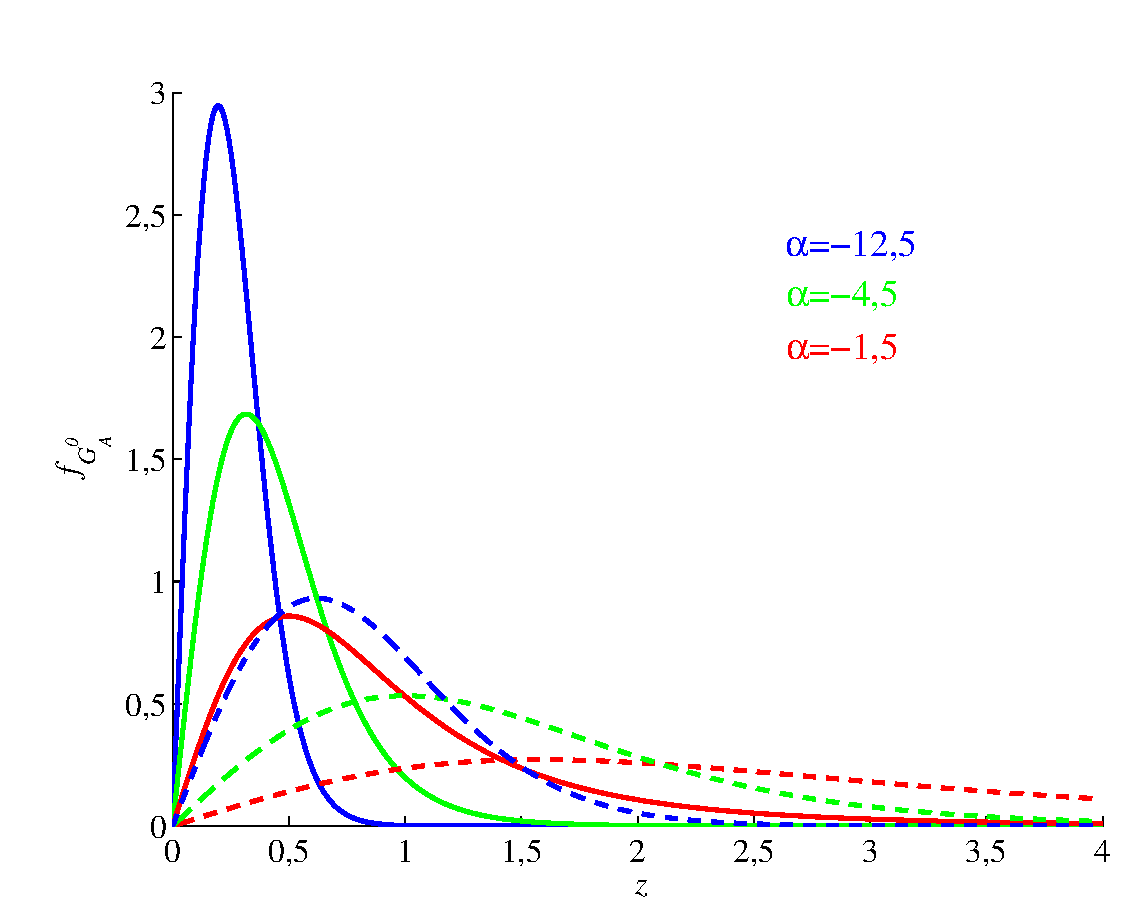
\includegraphics[scale=.65]{figures/fig1.eps}}\\
%\subfloat[]{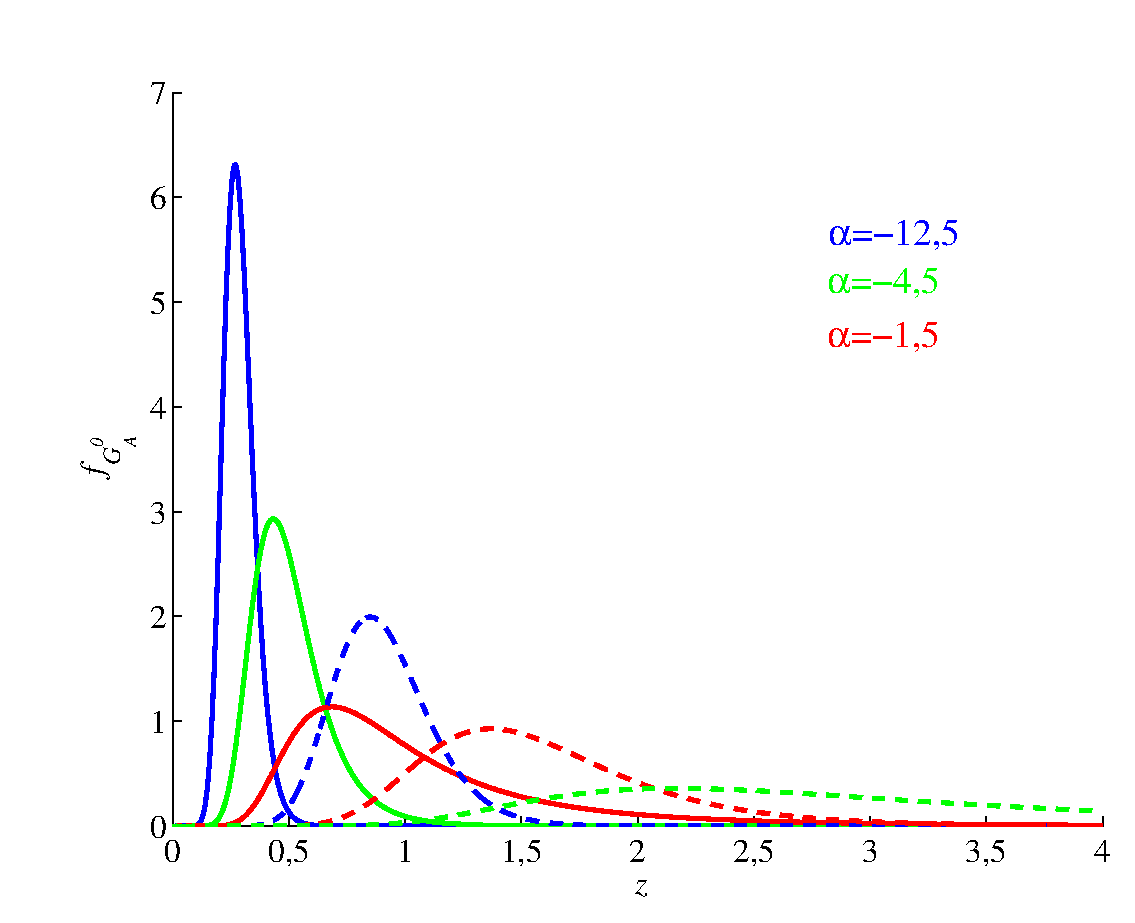
\includegraphics[scale=.65]{figures/fig2.eps}}
%\caption{ Curvas de funções de probabilidade: (a) exemplo 1, (b) exemplo 2.} \label{Fig:1}
%\end{figure}
\include{cap3}
\chapter{Cenário avaliado}
\label{CAP4}

Neste capítulo, é apresentado o ambiente Apache Hadoop que foi idealizado, no qual é baseado em uma metodologia exploratória e experimental. Esse ambiente busca prover um auxílio ao usuário para que ele possa realizar testes antes de montar um ambiente real.

O ambiente Apache Hadoop consiste em alguns \textit{softwares} gratuitos nos quais foram necessários realizar os \textit{downloads}, tais como: Ubuntu-server 16.04, java-8, Hadoop-2.9.1, Ubuntu-Desktop-16.04, virtual-box e o kali-Linux-x64. A figura \ref{Fig:EstruturaGeraldoAmbiente}, ilustrada no primeiro capítulo tenta dar uma visão geral do ambiente proposto. Os \textit{downloads} dos \textit{softwares} citados anteriormente são ferramentas essenciais para o desenvolvimento deste trabalho, o procedimento de instalação também é bastante simples, porém, um pouco demorado considerando o \textit{hardware} da máquina principal e tendo em vista que tudo estará dependendo apenas de uma máquina.

\begin{comment}
De inicio foi instalado o virtual-box na máquina local, em seguida foi criado uma máquina virtual com o ubuntu-server na sua instalação padrão com a instalação do openSSH Server que servirá para comunicação entre os nós do cluster. Após isso, foi instalado o java na versão 8, em seguida basta clonar essa máquina criada e escolher ela como o master e os demais como os slaves. Após isso foi necessário criar uma chave pública e um usuário e senha para cada nó.
\end{comment}

\section{Processo de instalação}

O processo de criação de uma máquina virtual com o \textit{software} virtual-box é bem simples, basta abrir o \textit{software} e depois clicar no botão 'novo', após isso é só escolher o nome e a quantidade de memória que deseja alocar para a máquina virtual. Com isso, basta seguir os procedimentos de instalação do sistema operacional, tais como, idioma, hora, usuário e senha.

\subsubsection{Instalação do Ubuntu Server}

Um cluster pode ser criado com qualquer sistema operacional, inclusive ele pode conter máquinas com diferentes sistemas operacionais, visto que, a comunicação é realizada pela rede via ssh, sendo assim, optou-se pelo sistema operacional Ubuntu server, pois o mesmo é gratuito e de código aberto. 

Ao concluir a instalação do Ubuntu server, é necessário fazer algumas outras instalações no sistema operacional, tais como, o java e o openSSH. Concluindo essas instalações é necessário desabilitar o ipv6 para poder utilizar o endereço 10.0.0.0 como \textit{network}. Para desabilitar o ipv6 bastar ir no caminho /etc/sysctl.config e adicionar as seguintes linhas:

\begin{figure}[htbp!] \begin{center}
	% fbox faz uma borda ao redor do seu argumento
    \fbox{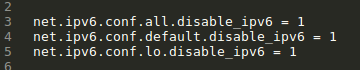
\includegraphics[width=0.80\linewidth]{figures/disableIpv6}}
    \caption{Desabilitando o Ipv6}
	\small{Fonte - (próprio autor, 2018)}
	\label{Fig:Desabilitando o Ipv6}
	\end{center} \end{figure}

%http://blog.aloi.com.br/?p=284


Tendo o java instalado, o openSSH instalado e o ipv6 desabilitado, precisa-se criar uma chave para o SSH, que permite a conexão sem precisar digitar senha. Para criar a chave foi utilizado o comando: 'ssh-keygen -t rsa -P "" '. Após gerar a chave pública basta copiar para um arquivo chamado \textit{authorizedKeys}, isso tudo significa que está máquina aceitará a conexão de outra máquina que tenha a chave privada. Então, até este momento a configuração entre as máquinas do cluster está configurada. A próxima etapa é a instalação e configuração do \textit{framework} Apache Hadoop. 

\subsubsection{Instalação do framework Apache Hadoop}

Assim que concluir a instalação do Ubuntu server e as configurações necessárias, basta realizar o \textit{download} do Apache Hadoop, que pode ser encontrado no repositório da unicamp no seguinte link: \url{http://ftp.unicamp.br/pub/apache/hadoop/core/stable/}.

Logo que o \textit{download} for conluído é necessário editar o arquivo de configuração do usuário, chamado de .bashrc, neste arquivo são adicionados as variáveis de ambiente do Hadoop ao PATH, com as seguintes linhas de código: \\

\begin{figure}[htbp!] \begin{center}
	% fbox faz uma borda ao redor do seu argumento
    \fbox{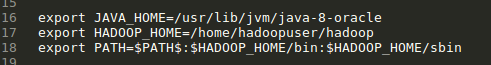
\includegraphics[width=0.80\linewidth]{figures/variaveisBashrc}}
    \caption{Adicionando variáveis do Apache Hadoop ao path}
	\small{Fonte - (próprio autor, 2018)}
	\label{Fig:Adicionando variaveis do hadoop ao path}
	\end{center} 
\end{figure}


Concluindo essa etapa, basta clonar a máquina \textit{master} criada e renomear as demais máquinas, transformando-as em \textit{slaves}, pois isso economiza tempo e as configurações já estão todas certas. No momento de realizar o clone, deve-se selecionar o \textit{checkbox} para reinicializar o endereço MAC da nova máquina, após isso basta configurar o IP de cada \textit{slave} para que eles fiquem na mesma faixa de IP, ou seja, na mesma rede.

Após isso, começa a instalação do Apache Hadoop, as configurações própriamente dita, entrando no seguinte caminho, hadoop/etc/hadoop e editando o arquivo hadoop-env.sh, pois ele é comum tanto para o \textit{master} quanto para os \textit{slaves}, neste arquivo é necessário colocar o caminho que o java esta instalado na máquina, para descobrir isso, basta digitar o comando "env | grep JAVA", neste caso a saída foi "JAVA\_HOME=/usr/lib/jvm/java-8-oracle".

O \textit{framework} Apache Hadoop contém diversos arquivos de configuração, esses arquivos são do tipo XML e especificam como o \textit{framework} irá conduzir suas tarefas. Para configurar o Apache Hadoop foi necessário editar alguns arquivos XML, tais como: 

\begin{itemize}

\item \textbf{Core-site.xml:} Este arquivo define as configurações de qual host será o \textit{master} no cluster Hadoop.

\begin{comment}
\begin{center}
	\lstinputlisting[caption = {core-site}, label=teste]{figures/core-site.xml}
\end{center}
\end{comment}

\begin{comment}
\begin{figure}[htbp!] 
	\begin{center}
	% fbox faz uma borda ao redor do seu argumento
	\fbox{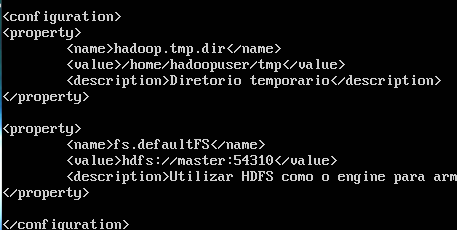
\includegraphics[width=0.80\linewidth]{figures/configCore-site}}
	\caption{Configuração do Core-site.xml}
    \small{Fonte - (proprio autor, 2018)}
	\label{Fig:Configuração do core-site.xml}
	\end{center} 
\end{figure}
\end{comment}

\item \textbf{Hdfs-site.xml:} É o \textit{filesystem} e nele são configurados as quantidades de replicações que o Hadoop HDFS deve fazer, onde estão localizados os metadados que o namenode utiliza para gerenciar o cluster e onde estão sendo armazenados os arquivos dentro do HDFS.

\begin{comment}
\begin{figure}[htbp!] 
	\begin{center}
	% fbox faz uma borda ao redor do seu argumento
	\fbox{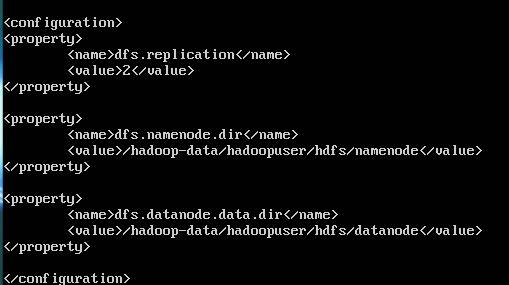
\includegraphics[width=0.80\linewidth]{figures/confighdfs-site}}
	\caption{Configuração do Hdfs-site.xml}
	\small{Fonte - (proprio autor, 2018)}
	\label{Fig:Configuração do hdfs-site.xml}
	\end{center} 
\end{figure}
\end{comment}

\item \textbf{Mapred-site.xml:} Este arquivo não existe por padrão, copia-se ele do mapred-site.xml.template e depois edita. Este arquivo define as configurações responsável por qual \textit{framework} que vai rodar os \textit{Jobs} do MapReduce, neste caso é o Yarn. Como o Yarn funciona com o conceito de container, é necessário alocar memória tanto para a operação de \textit{map} quanto para operação de \textit{reduce}.

\begin{comment}
\begin{figure}[htbp!] 
	\begin{center}
	% fbox faz uma borda ao redor do seu argumento
	\fbox{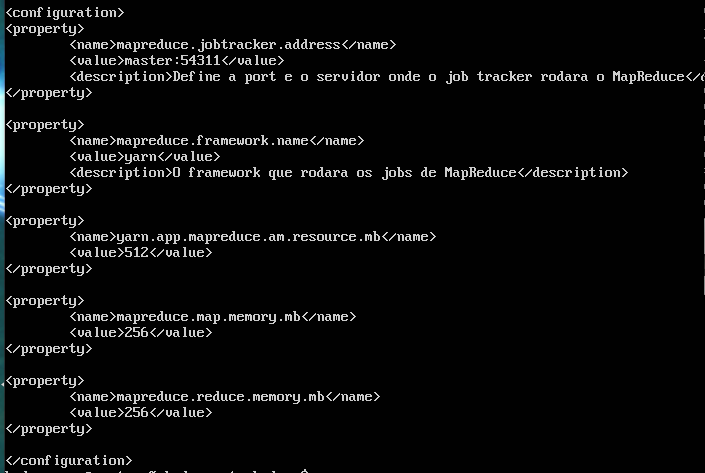
\includegraphics[width=0.90\linewidth]{figures/configmapred-site}}
	\caption{Configuração do mapred-site.xml}
	\small{Fonte - (proprio autor, 2018)}
	\label{Fig:Configuração do mapred-site.xml}
	\end{center} 
\end{figure}
\end{comment}


\item \textbf{Yarn-site.xml:} Como o Yarn será o gerenciador, ele precisa ser configurado, com isso, deve-se configurar qual serviço irá realizar o \textit{shuffle} dos dados do Apache Hadoop, qual a quantidade máxima e mínima de memória será alocada para as sua tarefas, quais portas do Yarn ficará ouvindo, e entre outras coisas.\footnote{shuffle: o algoritmo faz uma busca em todos os nós e após a coleta, junta tudo e traz um resultado}. 

\begin{comment}
As figuras \ref{Fig:Configuração do yarn-site.xml} e \ref{Fig:Configuração do yarn-site.xml-2} demonstram as configurações do yarn-site.xml.
\end{comment}

\begin{comment}
\begin{figure}[htbp!] \begin{center}
	% fbox faz uma borda ao redor do seu argumento
	\fbox{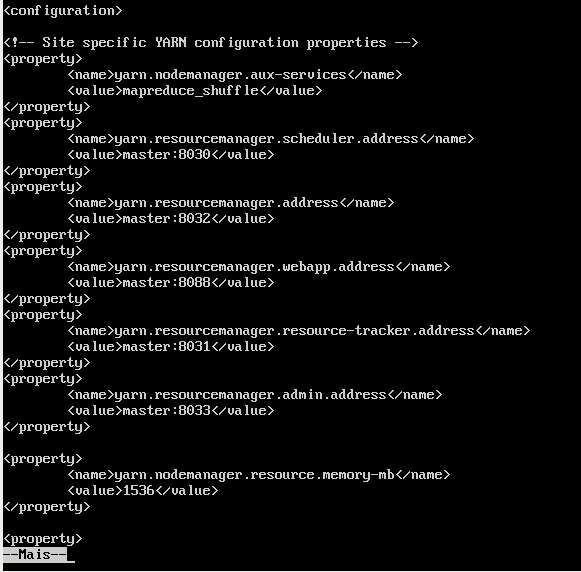
\includegraphics[width=0.80\linewidth]{figures/configYarn-site01}}
	\caption{Configuração do yarn-site.xml}
	\small{Fonte - (proprio autor, 2018)}
	\label{Fig:Configuração do yarn-site.xml}
	\end{center} \end{figure}

\begin{figure}[htbp!] \begin{center}
	% fbox faz uma borda ao redor do seu argumento
	\fbox{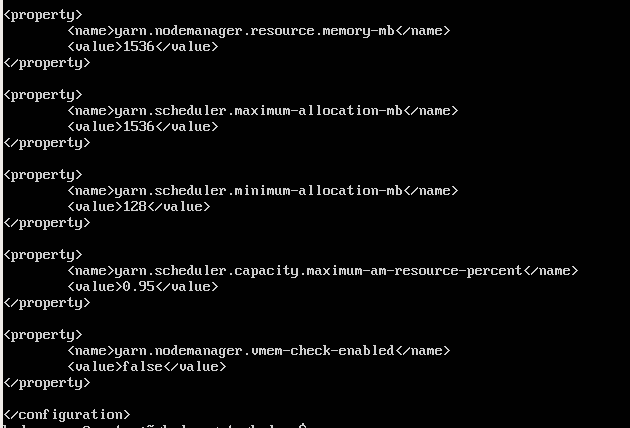
\includegraphics[width=0.80\linewidth]{figures/configYarn-site02}}
	\caption{Configuração do yarn-site.xml}
	\small{Fonte - (proprio autor, 2018)}
	\label{Fig:Configuração do yarn-site.xml-2}
	\end{center} \end{figure}
\end{comment}

\item \textbf{Arquivo de Slaves:} Neste arquivo chamado de \textit{slaves} ele não possui extensão, é o local onde deve-se colocar os nomes das máquinas configuradas no cluster que irão utilizar os serviços do Apache Hadoop. Neste caso o arquivo \textit{slaves} foram acrescentados os seguintes nome: \textit{master}, \textit{slave1}, \textit{slave2} e \textit{slave3}.

\end{itemize}

Após toda a configuração do Apache Hadoop na máquina \textit{master} alguns arquivos precisam ser copiados para os \textit{slaves}, sendo assim, utilizando o comando scp do terminal linux do \textit{master} pode-se copiar os arquivos, core-site.xml, hdfs-site.xml e o yarn-site.xml para os \textit{slaves}. De posse desses arquivos nos diretórios certos, basta executar o seguinte comando: "hdfs namenode -format". Este comando irá formatar o sistema de arquivos, finalizado e com uma mensagem de sucesso. A inicialização do Apache Hadoop pode ser realizada com o seguinte comando: "start-dfs.sh", para isso deve-se está dentro do diretório hadoop/etc/hadoop. Após iniciar o Hadoop é necessário iniciar o Yarn, com o seguinte comando: yarn-start.sh. Feito isso, para saber se está tudo funcionando basta executar o comando jps, como ilustrado nas figuras \ref{Fig:Comando jps Slave} e \ref{Fig:Comando jps Master}.

\begin{figure}[htbp!] \begin{center}
	% fbox faz uma borda ao redor do seu argumento
	\fbox{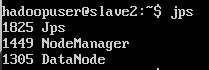
\includegraphics[width=0.40\linewidth]{figures/jpsSlave}}
	\caption{Comando jps Slave}
	\small{Fonte - (próprio autor, 2018)}
	\label{Fig:Comando jps Slave}
	\end{center} \end{figure}
    
    \begin{figure}[htbp!] \begin{center}
	% fbox faz uma borda ao redor do seu argumento
	\fbox{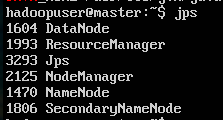
\includegraphics[width=0.40\linewidth]{figures/jpsMaster}}
	\caption{Comando jps Master}
	\small{Fonte - (próprio autor, 2018)}
	\label{Fig:Comando jps Master}
	\end{center} \end{figure}

Como ilustrado na figura \ref{Fig:Comando jps Master}, o nó \textit{master} contém mais processos em relação ao nó \textit{slave}, pois o \textit{master} é o gestor da aplicação, ele irá gerenciar e coordenar as tarefas.

\subsubsection{Cluster Hadoop}

Após completar todas as instalações necessárias, que são desde a criação da primeira máquina virtual até a instalação e configuração do \textit{framework} Apache Hadoop, tem-se o cluster funcionando. Para verificar se o cluster está realmente funcionando foi executado uma tarefa, e a partir de outra máquina acessando o endereço \url{10.0.0.1:8088/cluster/nodes} é possivel navegar e visualizar a interface do Yarn que é executada na porta 8088, enquanto que, o endereço \url{10.0.0.1:50070/dfshealth.html} na porta 50070 é possível visualizar o estado do cluster, como ilustram as figuras \ref{Fig:Interface do Yarn} e \ref{Fig:Estado do Cluster}.

\begin{figure}[htbp!] \begin{center}
	% fbox faz uma borda ao redor do seu argumento
	\fbox{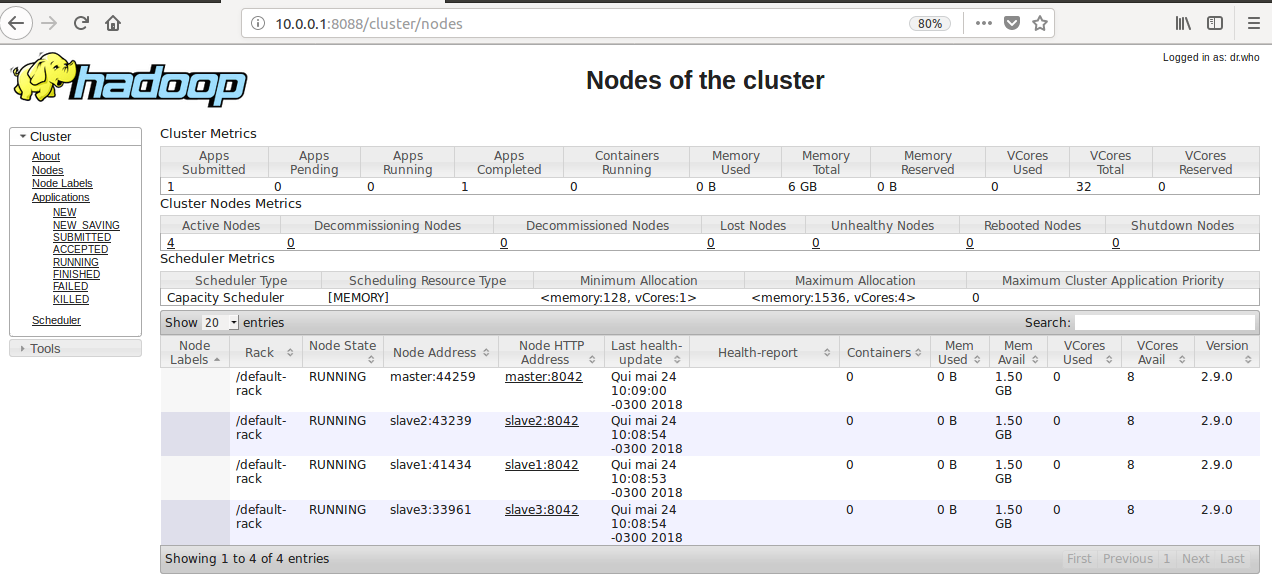
\includegraphics[width=1\linewidth]{figures/interfaceYarn}}
	\caption{Interface do Yarn}
	\small{Fonte - (próprio autor, 2018)}
	\label{Fig:Interface do Yarn}
	\end{center} \end{figure}
    
    \begin{figure}[htbp!] \begin{center}
	% fbox faz uma borda ao redor do seu argumento
	\fbox{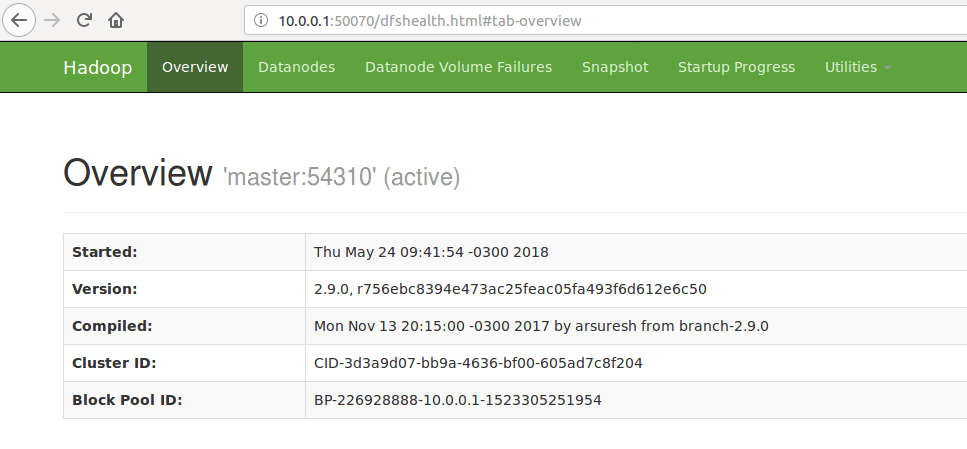
\includegraphics[width=1\linewidth]{figures/estadoDoCluster}}
	\caption{Estado do Cluster}
	\small{Fonte - (próprio autor, 2018)}
	\label{Fig:Estado do Cluster}
	\end{center} \end{figure}


Vale salientar que o acesso as intefaces devem ser realizadas por uma máquina que esteja na mesma rede do cluster. Sendo assim, esse acesso foi realizado pela máquina atacante, que está configurada na mesma rede. Com estes painéis é possível visualizar toda as funcionalidades dos nós, tais como: logs, estatísticas, quantidade de memória disponível e alocada, memória total, quais as tarefas foram executadas sem falhas, e entre outras funcionalidades.

\chapter{Experimentos e resultados}
\label{CAP5}

Neste capítulo são apresentados os experimentos realizados no ambiente montado, como os testes foram realizados e quais considerações foram adotadas. Em segurança da informção é muito importante saber se defender de um ataque, ou saber que está sendo atacado, porém, para identificar um ataque ou saber se defender dele, é necessário saber realizar um ataque.

Tendo isso mente, foram realizados três tentativas de ataques diferentes, nos quais são explicados nas seções sequintes. As boas práticas de segurança da informação ou segurança dos dados vão muito além de senhas e sistemas com \textit{firewalls}, a segurança dos dados consiste de uma política bem elaborada pelos responsáveis e com todos da equipe respeitando essa política.

Os experimentos seguem as boas práticas de um \textit{pentest}, ou seja, seguindo as etapas de \textit{scanner}, exploração, e entre outras etapas já citadas. Os experimentos seguiram a sequinte sequência: \textit{scanner}, recolhimento de informações, ataque e por fim boas práticas de segurança para minimizar os danos ou dificultar a ação dos \textit{hackers}, essas boas práticas de segurança são dicas para ser seguidas e com isso evitar maiores transtornos.

\section{Cenário I}

Neste primeiro cenário a ideia principal consiste em testar uma das funcionalidades do \textit{framework} Apache Hadoop, que é a tolerância a falhas, ou seja, o ataque será direcionado a um nó do cluster, com o intuito de sobrecarregá-lo, com isso, segundo a literatura do Apache Hadoop, ela diz que o \textit{framework} é tolerante a falhas, e nestes momentos ele sabe se comportar, em caso de um nó sobrecarregado ele consegue distribuir as suas tarefas para os demais nós do cluster, então considerando essa informação, foi sugerido um ataque de negação de serviço, ou seja, um DoS, que consiste em apenas uma máquina enviando pacotes de requisições para o nó, na tentativa de derrubá-lo ou sobrecarregá-lo.

Como explicado anteriormente, a vítima é um nó do cluster, enquanto que o atacante é uma máquina com o sistema operacional Kali Linux. Ao realizar o \textit{scanner} da rede com o comando "nmap -T4 -A -v 10.0.0.0/24", obteve-se os resultados apresentados nas figuras \ref{Fig:Scaneando a rede} e \ref{Fig:Scaneando a rede mais completo}.

Os resultados apresentados nas figuras \ref{Fig:Scaneando a rede} e \ref{Fig:Scaneando a rede mais completo}, ilustram muitas informações a respeito das vítimas. Este \textit{scanner} permite identificar qual o sistema operacional, qual a versão do \textit{kernel}, quais serviços estão rodando, quais as portas que estão abertas e qual o nível de dificuldade que o atacante irá encontrar ao tentar quebrar a segurança. Da figura \ref{Fig:Scaneando a rede mais completo} pode-se extrair que o sistema operacional usado pelo cluster é o Ubuntu Linux 3.x ou 4.x e o \textit{kernel} 3.x ou 4.x.

Como qualquer sistema que esteja na internet está sujeito a um ataque de negação de serviço e tendo em vista, que a proposta deste primeiro ataque é verificar como o cluster Hadoop se comporta quando está sofrendo uma sobrecarga, tem-se então o cenário ideal para realizar um DoS.

O \textit{software} utilizado para realizar o ataque foi o HPING, que é um \textit{software} muito poderoso quando se trata de ataque de DoS, sendo assim, ao acessar o kali linux (máquina atacante), do terminal foram executados os seguintes comandos: "hping3 10.0.0.2 -p 80 -S --faster --rand-source". Com esse comando o atacante estará enviando 10 pacotes por segundo para a vítima com o IP 10.0.0.2, utilizando a porta 80. Esses pacotes enviados funcionam da seguinte forma:

\begin{enumerate}
	\item O cliente envia uma solicitação de conexão, com um pacote TCP sem dados, possuindo o flag de SYN ligado e os demais desligados. Por causa da presença do flag de SYN, este pacote é conhecido como pacote SYN.
	
	\item Se o servidor quiser e puder atender, devolve um pacote ao cliente ainda sem dados, com os flags de SYN e de ACK ligados. Está segunda etapa é conhecida como SYN/ACK.
	
	\item Se o cliente ainda quiser manter a conexão, devolve ao servidor um terceiro pacote sem dados, apenas com o flag de ACK ligado (SYN desligado).
\end{enumerate}

Somente após a terceira etapa é que os dados podem ser trocados. Quando o cliente realiza uma requisição ao servidor, o servidor aloca memória para a requisição do cliente e para a resposta, isso é chamado de \textit{handshake} de três vias, ou seja, o \textit{3way handshake}. O não cumprimento da segunda etapa por parte do cliente consome a memória alocada do servidor, sendo assim, muitos pacotes enviados o servidor irá ficar sobrecarregado e não conseguirá responder.

Os ataques foram realizados da seguinte forma: Primeiro foi executada uma tarefa de exemplo do Hadoop, dai mediu-se o tempo gasto pelo Hadoop para concluir essa tarefa, sem executar nenhum ataque. Após isso, iniciou-se os ataques com o tempo sendo cronometrado e executando a mesma tarefa, a tabela \ref{dadosDoDDOS} demonstra os dados avaliados.


\begin{figure}[htbp!] \begin{center}
% fbox faz uma borda ao redor do seu argumento
\fbox{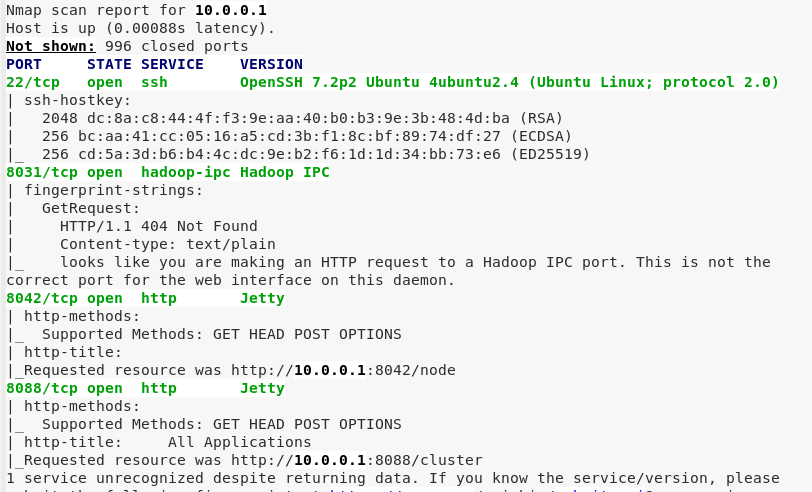
\includegraphics[width=0.80\linewidth]{figures/scaneamentoCompleto01}}
\caption{Scaneando a rede}
\small{Fonte - (próprio autor, 2018)}
\label{Fig:Scaneando a rede}
\end{center} \end{figure}

\begin{figure}[htbp!] \begin{center}
% fbox faz uma borda ao redor do seu argumento
\fbox{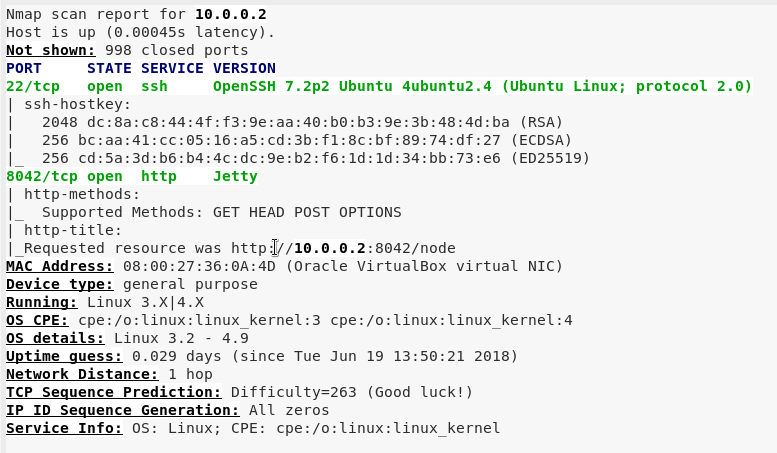
\includegraphics[width=0.80\linewidth]{figures/scaneamentoCompleto02}}
\caption{Scaneando a rede mais completo}
\small{Fonte - (próprio autor, 2018)}
\label{Fig:Scaneando a rede mais completo}
\end{center} \end{figure}

\newpage

% ######## init table ########
\begin{table}[h]
 \centering
% distancia entre a linha e o texto
 {\renewcommand\arraystretch{1.25}
 \caption{Dados do ataque DoS}
 \label{dadosDoDDOS}
 \begin{tabular}{ l l l }
  \cline{1-1}\cline{2-2}\cline{3-3}  
    \multicolumn{1}{|p{3.150cm}|}{\textbf{Duração do ataque (minutos)} \centering } &
    \multicolumn{1}{p{4.500cm}|}{\textbf{Tempo de execução da tarefa hadoop (segundos)} \centering } &
    \multicolumn{1}{p{2.350cm}|}{\textbf{Quantidade de pacotes enviados} \centering }
  \\  
  \cline{1-1}\cline{2-2}\cline{3-3}  
    \multicolumn{1}{|p{3.150cm}|}{0 \centering } &
    \multicolumn{1}{p{4.500cm}|}{147,892 \centering } &
    \multicolumn{1}{p{2.350cm}|}{0 \centering }
  \\  
  \cline{1-1}\cline{2-2}\cline{3-3}  
    \multicolumn{1}{|p{3.150cm}|}{5 \centering } &
    \multicolumn{1}{p{4.500cm}|}{178,673 \centering } &
    \multicolumn{1}{p{2.350cm}|}{8234110 \centering }
  \\  
  \cline{1-1}\cline{2-2}\cline{3-3}  
    \multicolumn{1}{|p{3.150cm}|}{10 \centering } &
    \multicolumn{1}{p{4.500cm}|}{180,754 \centering } &
    \multicolumn{1}{p{2.350cm}|}{13546404 \centering }
  \\  
  \cline{1-1}\cline{2-2}\cline{3-3}  
    \multicolumn{1}{|p{3.150cm}|}{15 \centering } &
    \multicolumn{1}{p{4.500cm}|}{189,357 \centering } &
    \multicolumn{1}{p{2.350cm}|}{20157836 \centering }
  \\
  \cline{1-1}\cline{2-2}\cline{3-3}  
    \multicolumn{1}{|p{3.150cm}|}{20 \centering } &
    \multicolumn{1}{p{4.500cm}|}{212,469 \centering } &
    \multicolumn{1}{p{2.350cm}|}{23817843 \centering }
    \\
  \hline

 \end{tabular} }
\end{table}


\begin{figure}[htbp!] \begin{center}
% fbox faz uma borda ao redor do seu argumento
\fbox{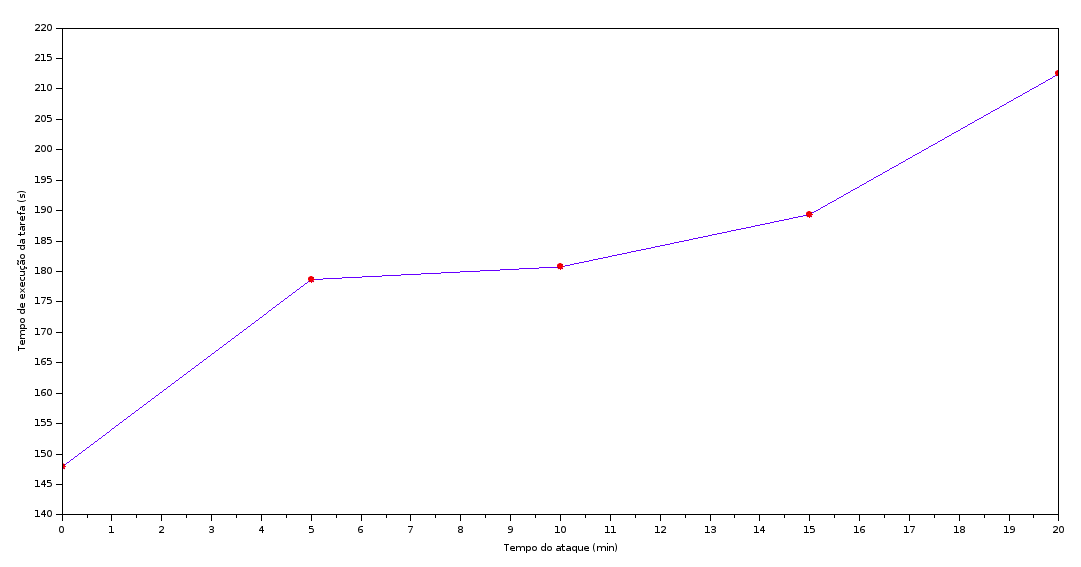
\includegraphics[width=1.0\linewidth]{figures/graficoDOS}}
\caption{Gráfico do DoS}
\small{Fonte - (próprio autor, 2018)}
\label{Fig:grafico do dos}
\end{center} \end{figure}

Levando em consideração que esse ataque é composto por apenas uma máquina e que existem algumas limitações de \textit{hardware}, tendo isso em mente, pode-se perceber que houve uma pertubação no meio fazendo com que o \textit{framework} demorasse mais tempo para concluir sua tarefa. De acordo com os dados percebe-se que se existissem mais máquinas enviando pacotes para um determinado nó do cluster ele ficaria altamente sobrecarregado, sendo assim as tarefas do cluster demorariam mais tempo para serem executadas, ou seja, quanto mais tempo o atacante passou enviando pacotes, mais tempo a tarefa demorou a ser concluída, isso pode ser uma dor de cabeça para empresas que precisam de resultado rápido para tomar decisões.

A figura \ref{Fig:grafico do dos} exibe uma função quase linear, ou seja, a medida que o ataque de negação de serviço demora, aumenta também o tempo de execução da tarefa pelo Hadoop, sem contar que durante a executação da tarefa mediante ataque foi percebido que o \textit{framework} Hadoop teve que 'matar' alguns dos seus processos para poder executar a tarefa proposta, liberando recursos para finalizar o \textit{Job}, enquanto estava sob ataques DoS.

Levando em consideração que esse ataque é realizado em pequena escala, ou seja, apenas de um host para outro determinado host e em um ambiente controlado. Pensando em um ambiente de produção de uma grande empresa e com milhares de hosts, esse ataque poderia causar sérios danos a infraestrutura da empresa escolhida.

\subsubsection{Boas práticas de segurança}

Sabendo que nenhum sistema está completamente protegido e que eles podem eventualmente sofrer algumas falhas, as boas práticas de segurança em ambiente Hadoop propõem a utilização de \textit{softwares} externos ao ambiente Hadoop, ou seja, proteger a rede de requisições falsas, evitando esses ataques de DoS, existem diversas maneiras para se defender de uma ataque DoS, tais como, implantação de um \textit{firewall} que filtre requisições falsas, assim seria possível saber quando o cluster estivesse sendo atacado por um ataque DoS. Existe também os Sistemas de Detecção de Intrusos.

Os IDS são usados para detectar vários tipos de comportamentos maliciosos que podem comprometer a segurança e a confiabilidade de um sistema. Eles incluem ataques pela rede contra serviços vulneráveis, ataques baseados em uma estação, como aumento de privilégio, logins não autorizados e \textit{malware}. Os IDS captam dados da rede e aplicam suas regras a esses dados ou detectam anomalias neles. Dependendo das configurações podem ser acionados alertas.




\newpage
\section{Cenário II}

Neste segundo cenário, a ideia principal consiste em explorar a vulnerabilidade de alguma porta aberta e a utilização de senhas padrões, como já houve o \textit{scanner} e com ele foram obtidos portas abertas, tais como, a 22, 8031, 8042, 8088. Como o protocolo ssh, porta 22, serve para que as máquinas do cluster façam sua comunicação ela foi a escolhida.

Explorando essa vulnerabilidade, espera-se obter acesso a um nó do cluster, pra isso, está prática pretende utilizar um conceito chamado de \textit{brute force}, ou seja, força bruta, que consiste em tentativas de acertar o usuário e a senha do ssh. Nesse teste foi utilizado uma \textit{wordlist} composta com diversas combinações de senhas e usuários. A comunicação realizada pelo ssh é feita tanto por uma chave privada quanto por senha.

Neste ataque foi utilizado o \textit{metasploit framework}, esse \textit{framework} é muito utilizado para a prática de força bruta, entre os protocolos que podem ser explorados, estão os protocolos ftp, telnet e o ssh, sendo assim, a exploração foi realizada com os seguintes comandos ilustrados na figura \ref{Fig:Comandos utilizados para o ataque de força bruta}. 

\begin{figure}[htbp!] \begin{center}
% fbox faz uma borda ao redor do seu argumento
\fbox{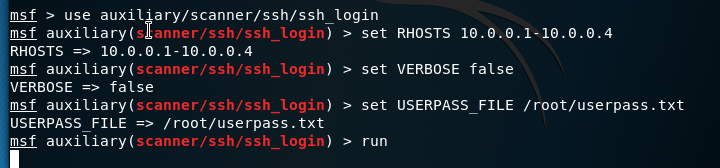
\includegraphics[width=0.70\linewidth]{figures/comandos}}
\caption{Comandos utilizados para o ataque de força bruta}
\small{Fonte - (próprio autor, 2018)}
\label{Fig:Comandos utilizados para o ataque de força bruta}
\end{center} \end{figure}

O primeiro comando "set RHOSTS 10.0.0.1-10.0.0.4", corresponde aos endereços para testar os usuários e senhas, ou seja, são as vítimas. O comando "set VERBOSE false". Quer dizer que só deve imprimir as tentativas que deu certo. O comando "set USERPASS\_FILE /root/userpass.txt", significa o caminho que está a \textit{wordlist}. Após a utilização destes comandos, o \textit{framework} testa todas as possibilidades inseridas no arquivo userpass.txt. Se o usuário e a senha corresponder a qualquer vítima, são exibidos a senha e o username, como ilustrado na figura \ref{Fig:Resultados do ataque de força bruta}.

\begin{figure}[htbp!] \begin{center}
% fbox faz uma borda ao redor do seu argumento
\fbox{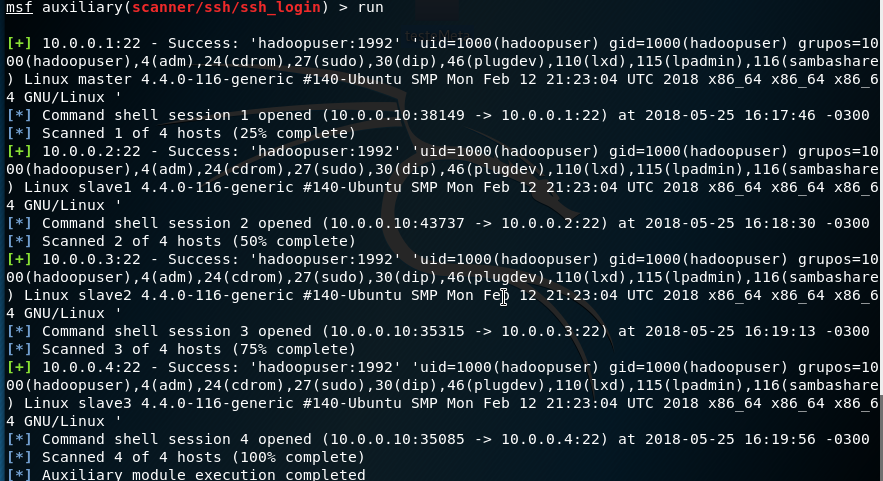
\includegraphics[width=0.80\linewidth]{figures/resultadoDoMetasploit}}
\caption{Resultados do ataque de força bruta}
\small{Fonte - (próprio autor, 2018)}
\label{Fig:Resultados do ataque de força bruta}
\end{center} \end{figure}

De acordo com os resultados obtidos na figura \ref{Fig:Resultados do ataque de força bruta}, percebe-se que ao tentar força bruta nos hosts com a faixa de IP 10.0.0.1 até 10.0.0.4, que é justamente o cluster, foram encontrados os usuários e as senhas dos mesmos. Percebe-se que o usuário do host 10.0.0.1 é 'hadoopuser' e a senha é '1992', para o restante dos hosts é a mesma senha e o mesmo usuário. Em posse desses dados é possível ter acesso via ssh aos nós do cluster ou até mesmo ao nó \textit{master} pela máquina atacante, como demonstrado na figura \ref{Fig:AcessoClusterPeloKali}.  Nela é demonstrado que do terminal do kali linux que é a máquina atacante, especificamente do terminal do metasploit, foi possível acessar o cluster.


\begin{figure}[htbp!] \begin{center}
% fbox faz uma borda ao redor do seu argumento
\fbox{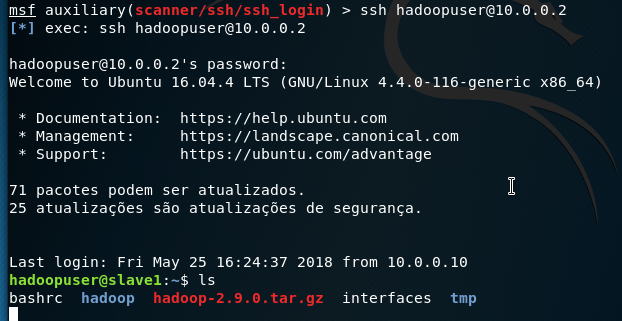
\includegraphics[width=0.80\linewidth]{figures/testandoUserPassword}}
\caption{Acessando o cluster pelo terminal do atacante}
\small{Fonte - (próprio autor, 2018)}
\label{Fig:AcessoClusterPeloKali}
\end{center} \end{figure}

Deve-se levar em consideração que esse ataque está em um ambiente controlado e que foi realizada uma engenharia social no proprietário para obter informações pessoais e com isso poder gerar uma \textit{wordlist} para tentar descobrir a senha e o usuário do cluster. Porém, obter informações de pessoas nos dias de hoje, não é uma tarefa muito difícil, tendo em vista que as redes sociais, sites de cadastros e outros meios na internet fornecem muitas informações nos quais os atacantes podem ter acesso de forma fácil e com isso poder fazer várias combinações e gerar arquivos com terabytes de senhas possíveis e tentar um ataque de força bruta. Conseguindo fazer isso e tendo acesso a um cluster ou até mesmo a uma aplicação o atacante pode usar sua imaginação e levar sérios prejuízos aos proprietários e as empresas.

\subsubsection{Boas práticas de segurança}

Em muitas configurações de e-mails, senhas de banco, senhas em geral, elas têm relação com o usuário ou com a empresa, estão relacionadas de alguma forma, seja por data de nascimento, por dia comemorativo, time de futebol, música, filmes, e entre outras relações que podem ser feitas para se gerar um dicionário e conseguir fazer uma força bruta para descobrir usuários e senhas.

Então, sabendo disso para o segundo cenário, as boas práticas de segurança consistem em senha fortes, contendo nomes minúsculos, maiúsculos, caracteres especiais e números, sem contar que ela deve ser grande no sentido de extensão, ou seja, uma senha com no mínimo quinze caracteres combinando os caracteres já citados. Isso dificulta um ataque de força bruta, e não ser relacionada com a empresa, ou seja, não deve conter nenhum nome ou qualquer caractere que se relacione com a empresa. 

Além das senhas fortes, uma outra prática importante seria limitar o acesso pelo ssh somente via chave pública realizando a configuração no OpenSSH, no caminho /etc/ssh/ssh\_config, para isso bastaria mudar para "no" as cláusulas PasswordAuthentication e UsePAM, além de gerar o par de chaves para os usuários e equipamentos envolvidos na autenticação (clientes e servidores). Habilitando o ssh para utilizar somente chaves públicas e privadas, há uma necessidade de proteger a privacidade dessas chaves, colocando-as em uma pasta na qual apenas o usuário root tenha acesso.

Essas práticas de senhas fortes e alterar a configuração do ssh são pouco praticadas entre empresas, pois no dia a dia os gestores necessitam rapidez e eficiência, não se preocupam com a segurança. Isso preocupa não só pela facilidade de descobrir as senhas ou burlar o sistema como também no uso de uma engenharia social efetuada pelo atacante para poder obter outros dados.

\newpage
\section{Cenário III}
Neste cenário a ideia principal consiste em realizar um ataque \textit{man in the middle} , ou seja, ficar no meio da comunicação entre os nós do cluster e conseguir executar tarefas, tais como: iniciar o nó, parar o nó, ter controle, logo, para o nó atacado a máquina atacante será o seu \textit{master}. Como explicado anteriormente, o ataque consiste em poluir a tabela ARP de um host e fazer com que ele se reporte ao atacante pensando que é o host verídico.

Para este ataque foram utilizadas algumas ferramentas, tais como: Ettercap, ubuntu 16.04, wireshark e foi necessário instalar o \textit{framework} Apache Hadoop nesta nova máquina atacante. A ideia inicial era instalar o Hadoop no sistema operacional Kali Linux, porém ao realizar os precedimentos de instalação houve diversos erros, alguns que poderiam comprometer os outros testes, com isso, optou-se por instalar o Ettercap e o wireshark em uma máquina Ubuntu, e realizar o ataque a partir dela, onde pra isso foi necessário colocar ela na rede, como ilustra a figura \ref{Fig:novoAmbiente}.

\begin{figure}[htbp!] \begin{center}
% fbox faz uma borda ao redor do seu argumento
\fbox{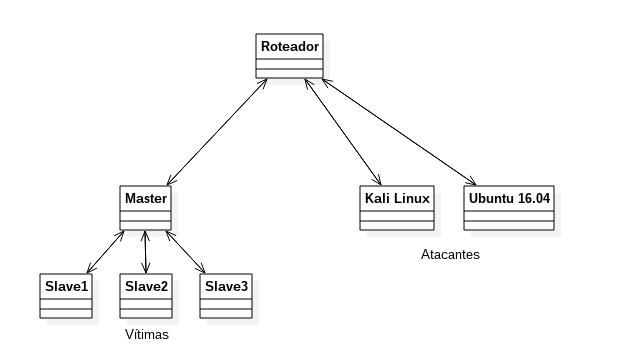
\includegraphics[width=0.80\linewidth]{figures/novoCenario}}
\caption{Visão geral do novo ambiente}
\small{Fonte - (próprio autor, 2018)}
\label{Fig:novoAmbiente}
\end{center} \end{figure}

Após isso, o ataque foi executado na seguinte ordem: Primeiro foi iniciado o nmap, para saber quais os hosts estão disponíveis na rede, com isso, foi obtido o resultado que ilustra a figura \ref{Fig:Scaneado a rede com nmap}. Selecionando a vítima, o próximo passo é iniciar o Ettercap, pois com ele será possível executar o arp-spoofing, que consiste em poluir a tabela ARP da vítima. A figura \ref{Fig:Interface do Ettercap} ilustra a interface da ferramenta, nela o primeiro passo é clicar em 'Sniff' e selecionar o modo 'Unified sniffing', após isso irá aparecer um \textit{PopUp} pedindo pra escolher a placa de rede, após isso basta ir na aba 'Hosts' e clicar em 'Scan for hosts' em seguida na mesma aba clica em 'Host List', depois desses passos serão listados os hosts da rede scaneada, com isso basta selecionar o host que será a vítima, clicar em target, ir na aba 'MITM' e selecionar a opção 'ARP poisoning', depois disso é só clicar em 'Start' que o ataque começa.

\begin{figure}[htbp!] \begin{center}
% fbox faz uma borda ao redor do seu argumento
\fbox{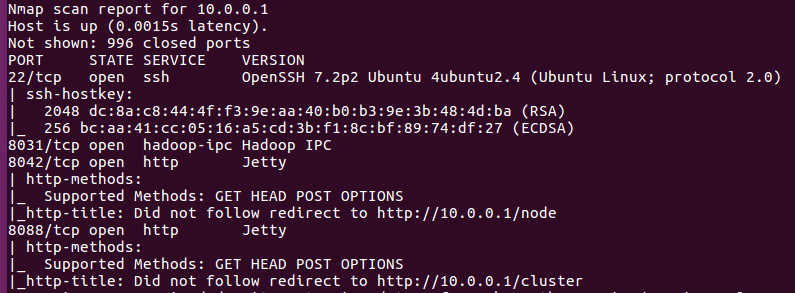
\includegraphics[width=0.80\linewidth]{figures/nmapNovoCenario}}
\caption{Scaneado a rede com nmap}
\small{Fonte - (próprio autor, 2018)}
\label{Fig:Scaneado a rede com nmap}
\end{center} \end{figure}

%%%%%%%%%%%%%%%%%%%%%%%%%%%%%%%%%%%%%%%%%%%%%%%%%%%%%%%%%%%%%%%

\begin{figure}[htbp!] \begin{center}
% fbox faz uma borda ao redor do seu argumento
\fbox{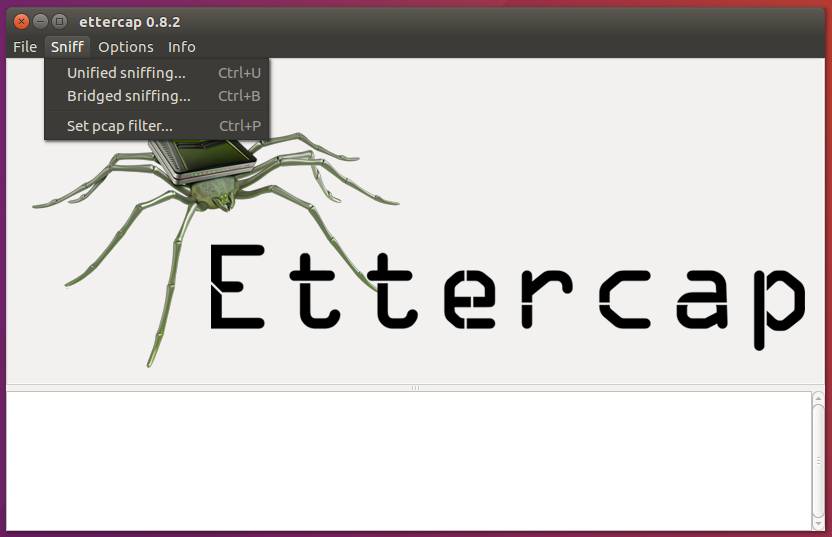
\includegraphics[width=0.80\linewidth]{figures/ettercap01}}
\caption{Interface do Ettercap}
\small{Fonte - (próprio autor, 2018)}
\label{Fig:Interface do Ettercap}
\end{center} \end{figure}

%AQUI É PRA EXPLICAR MAIS SOBRE A TABELA ARP

Como explicado anteriormente, esse ataque consiste em poluir a tabela ARP da vítima, ou seja, na tabela ARP contém todos os dados associados aos endereços IP e MAC, então ao realizar o envio dos dados do atacante para a tabela ARP da vítima ocorre a poluição da tabela, confundindo a vítima para que ela se comunique com o atacante pensando que está se comunicando com o \textit{master}, pois esse ataque foi direcionado a um nó do cluster, a vítima escolhida foi o \textit{slave1} com o endereço de IP 10.0.0.2. Para saber se o ataque está funcionando, o Hadoop foi iniciado no \textit{master}. Com isso, ao abrir o \textit{slave1} e digitar o comando "arp -a" ou "arp -n" pois esse comando serve para dizer qual o endereço MAC e IP o \textit{slave} está se comunicando. A figura \ref{Fig:Comando arp -n antes do ataque} ilustra o comando "arp -n" no \textit{slave1} antes do ataque, e a figura \ref{Fig:Comando arp -n durante o ataque} ilustra o comando "arp -n" no \textit{slave1} durante a execução do ataque \textit{man in the middle}.
%duas imagens aqui para fazer a visualização
%
\begin{figure}[htbp!] \begin{center}
% fbox faz uma borda ao redor do seu argumento
\fbox{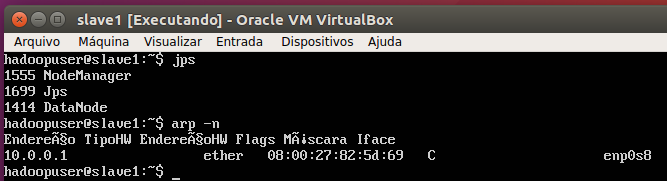
\includegraphics[width=0.90\linewidth]{figures/comandoarpAntesdoAtaque}}
\caption{Comando arp -n antes do ataque}
\small{Fonte - (próprio autor, 2018)}
\label{Fig:Comando arp -n antes do ataque}
\end{center} \end{figure}


\begin{figure}[htbp!] \begin{center}
% fbox faz uma borda ao redor do seu argumento
\fbox{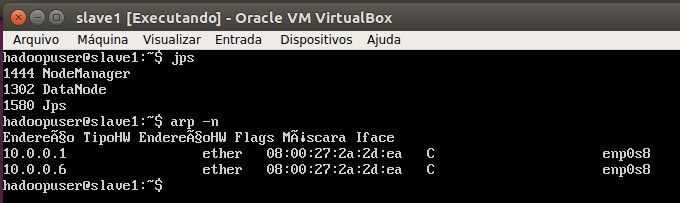
\includegraphics[width=0.90\linewidth]{figures/comandosDepoisAtaque}}
\caption{Comando arp -n durante o ataque}
\small{Fonte - (próprio autor, 2018)}
\label{Fig:Comando arp -n durante o ataque}
\end{center} \end{figure}


Como ilustram as figuras \ref{Fig:Comando arp -n antes do ataque} e \ref{Fig:Comando arp -n durante o ataque} ocorreu uma alteração no endereço MAC do nó \textit{master}, ou seja, o endereço MAC do nó \textit{master} passou a ser o endereço MAC do atacante como ilustra a figura \ref{Fig:Comando arp -n durante o ataque}. Com isso, o \textit{slave1} quando for se comunicar com o \textit{master} ele estará se comunicando com o atacante, pois o endereço MAC do atacante está associado ao IP do \textit{master}.

Para saber se o ataque está mesmo funcionando, ou seja, se o \textit{slave1} está mesmo se comunicando com o atacante ao invés de está se comunicando com o \textit{master}, basta acessar o atacante e tentar parar o nó \textit{slave1}, como ilustra a figura \ref{Fig:Stop Slave1}


\begin{figure}[htbp!] \begin{center}
% fbox faz uma borda ao redor do seu argumento
\fbox{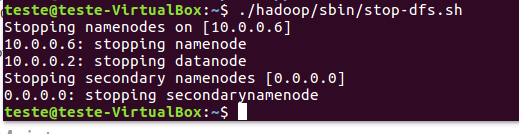
\includegraphics[width=0.90\linewidth]{figures/stopingSlave1}}
\caption{Stop Slave1}
\small{Fonte - (próprio autor, 2018)}
\label{Fig:Stop Slave1}
\end{center} \end{figure}

Como ilustra a figura \ref{Fig:Stop Slave1} percebe-se que o datanode com o IP 10.0.0.2 está stopping, ou seja, ele é parando, esse IP é justamente o IP do \textit{Slave1}, além disso ao acessar o \textit{Slave1} e verificar se está funcionando alguma aplicação percebe-se ao executar o comando jps, apenas duas aplicações estão funcionando, ao invés de três aplicações, como ilustra a figura \ref{Fig:Atividades Slave1 depois do Stop}.

\begin{figure}[htbp!] \begin{center}
% fbox faz uma borda ao redor do seu argumento
\fbox{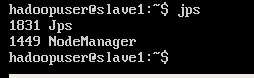
\includegraphics[width=0.72\linewidth]{figures/depoisDoStopPeloAtacante}}
\caption{Atividades Slave1 depois do Stop}
\small{Fonte - (próprio autor, 2018)}
\label{Fig:Atividades Slave1 depois do Stop}
\end{center} \end{figure}

Ao acessar o painel do Apache Hadoop e verificar a situação dos datanodes, percebe-se que o \textit{Slave1} não está funcionando, ou seja, o atacante conseguiu parar o datanode e com isso o ataque foi realizado com sucesso, como ilustra a figura \ref{Fig:painelDatanodeStop}.

\begin{figure}[htbp!] \begin{center}
% fbox faz uma borda ao redor do seu argumento
\fbox{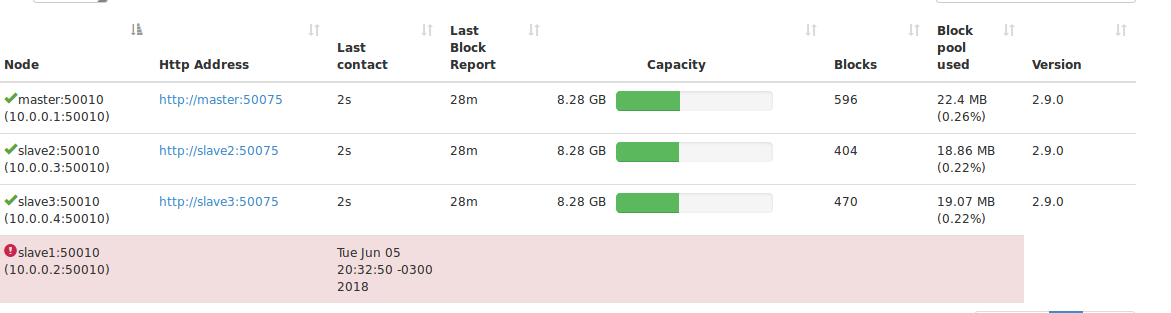
\includegraphics[width=0.90\linewidth]{figures/painelDatanodeStop}}
\caption{Painel Datanode Stop}
\small{Fonte - (próprio autor, 2018)}
\label{Fig:painelDatanodeStop}
\end{center} \end{figure}

Vale salientar que o atacante estava de posse das chaves do ssh para que o ataque funcionasse com perfeição, pois sem elas não seria possível ocorrer a comunicação entre a máquina atacante e o slave1. Sem as chaves do ssh, apenas era possível poliur a tabela ARP da vítima, mas não seria possível realizar o stop no DataNode.


Sendo assim, o \textit{man in the middle} foi realizado com sucesso, considerando que esse ataque está em um ambiente controlado, ele não dará nenhuma dor de cabeça, porém, se esse ataque fosse em larga escala, em um ambiente de produção? Seria uma dor de cabeça enorme para os desenvolvedores, sem contar que a empresa seria atingida.

\subsubsection{Boas práticas de segurança}

Durante um ataque \textit{man in the middle}, o host do atacante distribui seu próprio endereço MAC juntamente com seu endereço de IP em \textit{broadcast}, fazendo com que a vítima insira esses dados na sua tabela ARP. Visto isso, as boas práticas de segurança utilizadas neste cenário consistem em utilizar um Sniffer de pacotes na rede procurando as mensagens ARP que estão sendo enviadas aleatoriamente, ou seja, em \textit{broadcast}.

Uma outra maneira de se defender de um ataque MITM seria utilizando um IP estático, ou seja, fixar o IP e o endereço MAC do roteador na tabela ARP da vítima, pois quando o atacante enviasse seus dados IP e MAC em broadcast, querendo se passar pelo roteador, não iria funcionar, pois na tabela ARP da vítima já consta o IP e o MAC associados a outro host.

As chaves do ssh são de fundamental importância para que se possa ter acesso ao cluster, sendo assim, torna-se imprescindível que essas chaves sejam protegidas em uma pasta criptografada ou somente ao alcance do usuário root. Pois, em caso de não proteção corre-se o risco de comprometer todo o funcionamento do cluster.

O MITM é um ataque utilizado de várias formas, ele pode ser utilizado para roubar dados dos usuários através dos navegadores, capturar informações através da comunicação entre hosts e neste cenánio ele foi utlizado para ter acesso a um nó do cluster poluindo a tabela ARP da vítima. Sendo assim, para cada caso existem suas peculiaridades, porém, de forma geral uma maneira de identificar esse ataque é implantando um sniffer na rede ou sendo precavido e adicionando o IP e o MAC do roteador diretamente na tabela ARP da máquina utilizada.


%%%%%%%%%%%%%%%%%%%%%%%%%%%%%%%%%%%%%%%%%%%%%%%%%%%%%%%%%%%%%%

\chapter{Conclusão}
\label{CAP6}

\begin{comment}
Com o avanço das tecnologias muitos dados estão sendo gerados, grandes e pequenas empresas necessitam armazenar e processar essa imensidão de dados, porém, elas não estão dando as devidas importância para a segurança dos dados e das informações, podendo causar danos irreparáveis aos usuários.

Diversas empresas utilizam o ambiente hadoop para armazenar e processar grandes quantidades de dados, desta forma, este trabalho propos um ambiente simulado do hadoop para realizar testes de segurança e previnir danos com as boas praticas de segurança.

O ambiente criado proporciona ao desenvolvedor uma visão na qual ele ira poder realizar testes automatizados. Ele será capaz de testar a segurança do ambiente e prever falhas futuras. Este trabalho possui suas limitações quanto ao ambiente, tendo em vista que a máquina principal não possui um hardware excelente para o desenvolvimento de um cluster maior, mas as limitações foram controladas devido a simplificação na memoria disponivel ao cluster.
\end{comment}


%NOVA CONCLUSÃO
Com o avanço das tecnologias muitos dados estão sendo gerados, grandes e pequenas empresas necessitam armazenar e processar essa imensidão de dados, porém, elas não estão dando as devidas importância para a segurança dos dados e das informações, podendo causar danos irreparáveis aos usuários. Diversas empresas utilizam o ambiente Hadoop para armazenar e processar grandes quantidades de dados, desta forma, este trabalho propôs um ambiente simulado do Hadoop para realizar testes de segurança e previnir danos com as boas práticas de segurança, tendo em vista que o ambiente Apache Hadoop não vem com uma segurança mínima.

Como foi demonstrado durante este trabalho, o Hadoop por si só não trás nenhuma segurança, é necessário utilizar \textit{softwares} externos para blindar o ambiente Apache Hadoop. No primeiro cenário foi visto que, apenas uma máquina pôde causar lentidão no processo de um nó do cluster com um ataque DoS, no segundo cenário foi possível realizar um ataque de força bruta e conseguir descobrir a senha do ssh, sendo que o ssh é fundamental para o cluster, pois é através dele que ocorre a comunicação entre os nós. No terceiro cenário, foi possível realizar um MITM, conseguindo fazer com que um nó do cluster parasse de funcionar, prejudicando assim o cluster.

Como trabalhos futuros, pretende-se melhorar o ambiente nas questões de segurança de rede, com a implementação de uma segurança que proteja o ambiente contra ataques e realizar a troca de máquinas virtuais por \textit{raspberry pi}.

%\addcontentsline{toc}{section}{Referências}
\begin{thebibliography}{99}

\bibitem{livtex} ALOI BLOG. Instalar hadoop em ubuntu. Disponível em: \url{<http://blog.aloi.com.br/?p=284>}. Acesso em: 22 fev. 2018.

\bibitem{livtex} APACHE HADOOP. Welcome to apache hadoop. Disponível em: \url{<http://hadoop.apache.org/>}. Acesso em: 25 jan. 2018.

\bibitem{livtex} CANALTECH. Números curiosos do facebook: rede social gera mais de 500tb de dados por dia. Disponível em: \url{<https://canaltech.com.br/redes-sociais/facebook-gera-mais-500tb-de-dados-diariamente/>}. Acesso em: 04 jan. 2018.

\bibitem{livtex} CANALTECH. O que é dos e ddos?. Disponível em: \url{<https://canaltech.com.br/produtos/o-que-e-dos-e-ddos/>}. Acesso em: 15 fev. 2018.

\bibitem{livtex} DIFERENCIALTI. Segurança de dados: tudo que você precisa saber. Disponível em: \url{<https://blog.diferencialti.com.br/seguranca\-de-dados/>}. Acesso em: 05 jan. 2018.

\bibitem{livtex} DROIDHUB. Hadoop kerberos security. Disponível em: \url{<http://ngvtech.in/droidhub/hadoop\-kerberos-security/>}. Acesso em: 14 fev. 2018.

\bibitem{livtex} EXAME. Conteúdo digital dobra a cada dois anos no mundo. Disponível em: \url{<https://exame.abril.com.br/tecnologia/conteudo\-digital-dobra-a-cada-dois-anos-no-mundo/>}. Acesso em: 04 jan. 2018.

\bibitem{livtex} EXAME. Uma entrevista didática sobre big data. Disponível em: \url{<https://exame.abril.com.br/tecnologia/uma\-entrevista-didatica-sobre-big-data/>}. Acesso em: 05 jan. 2018.

\bibitem{livtex} GTA UFRJ. Kerberos. Disponível em: \url{<https://www.gta.ufrj.br/grad/02\_2/kerberos/>}. Acesso em: 13 fev. 2018.

\bibitem{livtex} HORTONWORKS. Apache hadoop yarn background and an overview. Disponível em: \url{<https://br.hortonworks.com/blog/apache\-hadoop-yarn-background-and-an-overview/>}. Acesso em: 09 fev. 2018.

\bibitem{livtex} HORTONWORKS. Apache hadoop yarn. Disponível em: \url{<https://br.hortonworks.com/apache/yarn/>}. Acesso em: 10 fev. 2018.

\bibitem{livtex} IBM. The four v's of big data. Disponível em: \url{<http://www.ibmbigdatahub.com/infographic/four\-vs-big-data>}. Acesso em: 08 jan. 2018.


\bibitem{livtex} IBM. Uma introdução ao hadoop distributed file system. Disponível em: \url{<https://www.ibm.com/developerworks/br/library/wa\-introhdfs/index.html>}. Acesso em: 29 jan. 2018.

\bibitem{livtex} INFOWESTER. Ataques dos (denial of service) e ddos (distributed dos). Disponível em: \url{<https://www.infowester.com/ddos.php>}. Acesso em: 16 fev. 2018.

\bibitem{livtex} INFOWESTER. Cluster: conceito e características. Disponível em: \url{<https://www.infowester.com/cluster.php>}. Acesso em: 17 jan. 2018.

\bibitem{livtex} JOSÉ GUILHERME LOPES. Hdfs e mapreduce: entenda a arquitetura do hadoop. Disponível em: \url{<http://joseguilhermelopes.com.br/hadoop\-entenda-arquitetura-hdfs/>}. Acesso em: 08 fev. 2018.

\bibitem{livtex} KALI LINUX. Our most advanced penetration testing distribution, ever.. Disponível em: \url{<https://www.kali.org/>}. Acesso em: 21 fev. 2018.

\bibitem{livtex} KAPLAN, Robert S.; NORTON, David P.. A estratégia em ação: Balanced scorecard. 4 ed.  Rio de Janeiro: Campus, 1997. 344 p.

\bibitem{livtex} LUME UFRJ. Simulação e estudo da plataforma hadoop mapreduce em ambientes heterogêneos. Disponível em: \url{<https://www.lume.ufrgs.br/bitstream/handle/10183/28331/000767852.pdf?sequence=1>}. Acesso em: 04 jan. 2018.

\bibitem{livtex} MAYER\-SCHÖNBERGER, Viktor; CUKIER, Kenneth. Big data: Como extrair volume, variedade, velocidade e valor da avalanche de informação cotidiana. 1 ed.  Brasil: Elsevier Brasil, 2014. 176 p.

\bibitem{livtex} MIDIAWEB. O que acontece na internet em um minuto?. Disponível em: \url{<http://www.midiaweb.com.br/o\-que-acontece-na-internet-em-um-minuto/>}. Acesso em: 04 jan. 2018.

\bibitem{livtex} MSBI. Big data, hadoop \- lesson 5 : namenode, datanode, job tracker, task tracker. Disponível em: \url{<https://lakshmana\-msbi.blogspot.com/2016/01/big-data-hadoop-lesson-5-namenode.html>}. Acesso em: 02 fev. 2018.

\bibitem{livtex} NINJA DO LINUX. Entenda o que é pentest (teste de intrusão), para que serve e como é feito. Disponível em: \url{<http://ninjadolinux.com.br/o\-que-e-pentest/>}. Acesso em: 19 fev. 2018.

\bibitem{livtex} NMAP. nmap security scanner. Disponível em: \url{<https://nmap.org/>}. Acesso em: 21 fev. 2018.

\bibitem{livtex} OSTEC. Iso 27002: boas práticas para gestão de segurança da informação. Disponível em: \url{<https://ostec.blog/padronizacao\-seguranca/iso-27002-boas-praticas-gsi>}. Acesso em: 05 jan. 2018.

\bibitem{livtex} PPLWARE. Redes sabe para que serve o protocolo arp?. Disponível em: \url{<https://pplware.sapo.pt/microsoft/windows/redes\-sabe-para-que-serve-o-protocolo-arp/>}. Acesso em: 18 fev. 2018.

\bibitem{livtex} PROFISSIONAISTI. Conhecendo o protocolo de rede kerberos. Disponível em: \url{<https://www.profissionaisti.com.br/2011/11/conhecendo\-o-protocolo-de-rede-kerberos/>}. Acesso em: 12 fev. 2018.

\bibitem{livtex} PROFISSÃO HACKER. Pentest. os testes de intrusão. Disponível em: \url{<http://profissaohacker.com/pentest/>}. Acesso em: 20 fev. 2018.

\bibitem{livtex} REPOSITORIO UNB. Modelo para estimar performance de um cluster hadoop. Disponível em: \url{<http://repositorio.unb.br/bitstream/10482/17180/1/2014\_josebeneditosouzabrito.pdf>}. Acesso em: 31 jan. 2018.

\bibitem{livtex} TECHMUNDO. Cerca de 100 bilhões de buscas são realizadas no google mensalmente. Disponível em: \url{<https://www.tecmundo.com.br/google/53852-cerca-de-100-bilhoes-de-buscas-sao-realizadas-no-google-mensalmente.htm>}. Acesso em: 04 jan. 2018.

\bibitem{livtex} TOTALCROSS. Banco de dados. relacional vs não relacional. Disponível em: \url{<http://www.totalcross.com/blog/banco\-de-dados-relacional-nao-relacional/>}. Acesso em: 17 jan. 2018.

\bibitem{livtex} WEBCHEATS. Ataque man\-in-the middle. Disponível em: \url{<http://www.webcheats.com.br/threads/6\-ataque-man-in-the-middle.2552630/>}. Acesso em: 17 fev. 2018.

\bibitem{livtex} WHITE, TOM. Hadoop the definitive guide: storage and analysis at internet scale. 4 ed.  USA: O reilly. 2015. 727 p.

\bibitem{livtex} DARKMOREOPS. Mitm man in the middle attack using kali linux. Disponivel em: \url{<https://www.darkmoreops.com/2015/11/16/mitm\-man-middle-attack-using-kali-linux/>}. Acesso em: 26 fev. 2018.

\bibitem{livtex} IMASTERS. Big data e hadoop – o que é tudo isso?. Disponível em: \url{<https://imasters.com.br/banco-de-dados/big-data-e-hadoop-o-que-e-tudo-isso>}. Acesso em: 19 fev. 2018.

\bibitem{livtex} TIINSIDE. Segurança de big data: como é feita?. Disponível em: \url{<http://tiinside.com.br/tiinside/seguranca/artigos-seguranca/25/07/2017/seguranca-de-big-data-como-e-feita/>}. Acesso em: 18 jun. 2018.

\bibitem{livtex} CIO. Segurança em big data é possível. Disponível em: \url{<http://cio.com.br/tecnologia/2016/04/01/seguranca-em-big-data-e-possivel/>}. Acesso em: 18 jun. 2018.

\bibitem{livtex} G1. Entenda o caso de edward snowden, que revelou espionagem dos eua. Disponível em: \url{<http://g1.globo.com/mundo/noticia/2013/07/entenda-o-caso-de-edward-snowden-que-revelou-espionagem-dos-eua.html>}. Acesso em: 04 jun. 2018.

\end{thebibliography}
%\chapter{Referencias}
\label{Referencias}


%%%% Estilo de citação ABNT e arquivo de bibitens (mybibliography.bib)
%\bibliographystyle{abnt-alf}
%\bibliographystyle{plain} %numeros na citação e bem organizado na referencia
%\bibliographystyle{abbrv} %numeros na citação e bem organizado na referencia
%\bibliographystyle{siam} %numeros na citação e bem organizado na referencia
%\bibliographystyle{apalike}
%\bibliography{ref}

%\apendice
%\chapter{Título do Apêndice}
\label{Apx:A}




\chapter{Exemplo do pacote Algorithm}
\label{Apx:B}


\begin{algorithm}[!h]
\caption{Estimador ML otimizado.}\label{Alg:MAXVER}
\begin{algorithmic}[1]
\STATE Inicializar o contador: $j\leftarrow 1$;%
\STATE Fixar o limiar de variação das estimativas: $e_{\mathrm{out}}\leftarrow 10^{-4}$;%
\STATE Fixar o número máximo de iterações: $N\leftarrow 1000$;%
\STATE Computar o ponto inicial: $\hat \gamma(0)$;%
\STATE Determinar o limiar inicial: $e_1 \leftarrow1000$;%
\STATE Estabelecer o valor inicial de $\alpha$: $\hat \alpha(0) \leftarrow -10^{-6}$;%
\WHILE{ $e_j \geq e_{\mathrm{out}}$ e $ j\leq M$}
    \STATE Solucionar $\hat \alpha_j\leftarrow {\arg \max}_{\alpha}\;{l_1(\alpha; \gamma_{j-1},\mathbf{z},n)}$;%
    \STATE Solucionar $\hat \gamma_j\leftarrow {\arg \max}_{\gamma}\;{l_2(\gamma; \alpha_j,\mathbf{z},n)}$;%
    \STATE $j\leftarrow j+1$
    \STATE Computar o critério de convergência: $e_j$;%
\ENDWHILE
\end{algorithmic}
\end{algorithm}


\end{document}